% Options for packages loaded elsewhere
\PassOptionsToPackage{unicode}{hyperref}
\PassOptionsToPackage{hyphens}{url}
\PassOptionsToPackage{dvipsnames,svgnames,x11names}{xcolor}
%
\documentclass[
  12pt]{article}
\usepackage{amsmath,amssymb}
\usepackage{iftex}
\ifPDFTeX
  \usepackage[T1]{fontenc}
  \usepackage[utf8]{inputenc}
  \usepackage{textcomp} % provide euro and other symbols
\else % if luatex or xetex
  \usepackage{unicode-math} % this also loads fontspec
  \defaultfontfeatures{Scale=MatchLowercase}
  \defaultfontfeatures[\rmfamily]{Ligatures=TeX,Scale=1}
\fi
\usepackage{lmodern}
\ifPDFTeX\else
  % xetex/luatex font selection
\fi
% Use upquote if available, for straight quotes in verbatim environments
\IfFileExists{upquote.sty}{\usepackage{upquote}}{}
\IfFileExists{microtype.sty}{% use microtype if available
  \usepackage[]{microtype}
  \UseMicrotypeSet[protrusion]{basicmath} % disable protrusion for tt fonts
}{}
\makeatletter
\@ifundefined{KOMAClassName}{% if non-KOMA class
  \IfFileExists{parskip.sty}{%
    \usepackage{parskip}
  }{% else
    \setlength{\parindent}{0pt}
    \setlength{\parskip}{6pt plus 2pt minus 1pt}}
}{% if KOMA class
  \KOMAoptions{parskip=half}}
\makeatother
\usepackage{xcolor}
\usepackage{color}
\usepackage{fancyvrb}
\newcommand{\VerbBar}{|}
\newcommand{\VERB}{\Verb[commandchars=\\\{\}]}
\DefineVerbatimEnvironment{Highlighting}{Verbatim}{commandchars=\\\{\}}
% Add ',fontsize=\small' for more characters per line
\usepackage{framed}
\definecolor{shadecolor}{RGB}{248,248,248}
\newenvironment{Shaded}{\begin{snugshade}}{\end{snugshade}}
\newcommand{\AlertTok}[1]{\textcolor[rgb]{0.94,0.16,0.16}{#1}}
\newcommand{\AnnotationTok}[1]{\textcolor[rgb]{0.56,0.35,0.01}{\textbf{\textit{#1}}}}
\newcommand{\AttributeTok}[1]{\textcolor[rgb]{0.13,0.29,0.53}{#1}}
\newcommand{\BaseNTok}[1]{\textcolor[rgb]{0.00,0.00,0.81}{#1}}
\newcommand{\BuiltInTok}[1]{#1}
\newcommand{\CharTok}[1]{\textcolor[rgb]{0.31,0.60,0.02}{#1}}
\newcommand{\CommentTok}[1]{\textcolor[rgb]{0.56,0.35,0.01}{\textit{#1}}}
\newcommand{\CommentVarTok}[1]{\textcolor[rgb]{0.56,0.35,0.01}{\textbf{\textit{#1}}}}
\newcommand{\ConstantTok}[1]{\textcolor[rgb]{0.56,0.35,0.01}{#1}}
\newcommand{\ControlFlowTok}[1]{\textcolor[rgb]{0.13,0.29,0.53}{\textbf{#1}}}
\newcommand{\DataTypeTok}[1]{\textcolor[rgb]{0.13,0.29,0.53}{#1}}
\newcommand{\DecValTok}[1]{\textcolor[rgb]{0.00,0.00,0.81}{#1}}
\newcommand{\DocumentationTok}[1]{\textcolor[rgb]{0.56,0.35,0.01}{\textbf{\textit{#1}}}}
\newcommand{\ErrorTok}[1]{\textcolor[rgb]{0.64,0.00,0.00}{\textbf{#1}}}
\newcommand{\ExtensionTok}[1]{#1}
\newcommand{\FloatTok}[1]{\textcolor[rgb]{0.00,0.00,0.81}{#1}}
\newcommand{\FunctionTok}[1]{\textcolor[rgb]{0.13,0.29,0.53}{\textbf{#1}}}
\newcommand{\ImportTok}[1]{#1}
\newcommand{\InformationTok}[1]{\textcolor[rgb]{0.56,0.35,0.01}{\textbf{\textit{#1}}}}
\newcommand{\KeywordTok}[1]{\textcolor[rgb]{0.13,0.29,0.53}{\textbf{#1}}}
\newcommand{\NormalTok}[1]{#1}
\newcommand{\OperatorTok}[1]{\textcolor[rgb]{0.81,0.36,0.00}{\textbf{#1}}}
\newcommand{\OtherTok}[1]{\textcolor[rgb]{0.56,0.35,0.01}{#1}}
\newcommand{\PreprocessorTok}[1]{\textcolor[rgb]{0.56,0.35,0.01}{\textit{#1}}}
\newcommand{\RegionMarkerTok}[1]{#1}
\newcommand{\SpecialCharTok}[1]{\textcolor[rgb]{0.81,0.36,0.00}{\textbf{#1}}}
\newcommand{\SpecialStringTok}[1]{\textcolor[rgb]{0.31,0.60,0.02}{#1}}
\newcommand{\StringTok}[1]{\textcolor[rgb]{0.31,0.60,0.02}{#1}}
\newcommand{\VariableTok}[1]{\textcolor[rgb]{0.00,0.00,0.00}{#1}}
\newcommand{\VerbatimStringTok}[1]{\textcolor[rgb]{0.31,0.60,0.02}{#1}}
\newcommand{\WarningTok}[1]{\textcolor[rgb]{0.56,0.35,0.01}{\textbf{\textit{#1}}}}
\usepackage{longtable,booktabs,array}
\usepackage{calc} % for calculating minipage widths
% Correct order of tables after \paragraph or \subparagraph
\usepackage{etoolbox}
\makeatletter
\patchcmd\longtable{\par}{\if@noskipsec\mbox{}\fi\par}{}{}
\makeatother
% Allow footnotes in longtable head/foot
\IfFileExists{footnotehyper.sty}{\usepackage{footnotehyper}}{\usepackage{footnote}}
\makesavenoteenv{longtable}
\usepackage{graphicx}
\makeatletter
\def\maxwidth{\ifdim\Gin@nat@width>\linewidth\linewidth\else\Gin@nat@width\fi}
\def\maxheight{\ifdim\Gin@nat@height>\textheight\textheight\else\Gin@nat@height\fi}
\makeatother
% Scale images if necessary, so that they will not overflow the page
% margins by default, and it is still possible to overwrite the defaults
% using explicit options in \includegraphics[width, height, ...]{}
\setkeys{Gin}{width=\maxwidth,height=\maxheight,keepaspectratio}
% Set default figure placement to htbp
\makeatletter
\def\fps@figure{htbp}
\makeatother
\setlength{\emergencystretch}{3em} % prevent overfull lines
\providecommand{\tightlist}{%
  \setlength{\itemsep}{0pt}\setlength{\parskip}{0pt}}
\setcounter{secnumdepth}{5}
% definitions for citeproc citations
\NewDocumentCommand\citeproctext{}{}
\NewDocumentCommand\citeproc{mm}{%
  \begingroup\def\citeproctext{#2}\cite{#1}\endgroup}
\makeatletter
 % allow citations to break across lines
 \let\@cite@ofmt\@firstofone
 % avoid brackets around text for \cite:
 \def\@biblabel#1{}
 \def\@cite#1#2{{#1\if@tempswa , #2\fi}}
\makeatother
\newlength{\cslhangindent}
\setlength{\cslhangindent}{1.5em}
\newlength{\csllabelwidth}
\setlength{\csllabelwidth}{3em}
\newenvironment{CSLReferences}[2] % #1 hanging-indent, #2 entry-spacing
 {\begin{list}{}{%
  \setlength{\itemindent}{0pt}
  \setlength{\leftmargin}{0pt}
  \setlength{\parsep}{0pt}
  % turn on hanging indent if param 1 is 1
  \ifodd #1
   \setlength{\leftmargin}{\cslhangindent}
   \setlength{\itemindent}{-1\cslhangindent}
  \fi
  % set entry spacing
  \setlength{\itemsep}{#2\baselineskip}}}
 {\end{list}}
\usepackage{calc}
\newcommand{\CSLBlock}[1]{\hfill\break\parbox[t]{\linewidth}{\strut\ignorespaces#1\strut}}
\newcommand{\CSLLeftMargin}[1]{\parbox[t]{\csllabelwidth}{\strut#1\strut}}
\newcommand{\CSLRightInline}[1]{\parbox[t]{\linewidth - \csllabelwidth}{\strut#1\strut}}
\newcommand{\CSLIndent}[1]{\hspace{\cslhangindent}#1}
\ifLuaTeX
\usepackage[bidi=basic]{babel}
\else
\usepackage[bidi=default]{babel}
\fi
\babelprovide[main,import]{spanish}
% get rid of language-specific shorthands (see #6817):
\let\LanguageShortHands\languageshorthands
\def\languageshorthands#1{}
\usepackage{makeidx}
\makeindex
\usepackage{graphicx}
\usepackage{tikz}
\usepackage{atbegshi}
\usepackage{amsthm}
\newtheorem{definition}{Definición}[section]

\AtBeginDocument{
    \AtBeginShipoutNext{
        \AtBeginShipoutUpperLeft{
            \put(\dimexpr\paperwidth/2-\textwidth/2\relax, -650){
                \makebox[\textwidth]{
                    
\includegraphics[width=0.6\textwidth]{cure_udelar.png}  % Adjust width as needed
                    \hfill
                    
\includegraphics[width=0.405\textwidth]{logoMEDIA.jpeg} % Make it 90% smaller
                }
            }
        }
    }
}

\usepackage{amsthm}
\usepackage{xcolor}
\ifLuaTeX
  \usepackage{selnolig}  % disable illegal ligatures
\fi
\usepackage{bookmark}
\IfFileExists{xurl.sty}{\usepackage{xurl}}{} % add URL line breaks if available
\urlstyle{same}
\hypersetup{
  pdftitle={Entrega: curso de datos extremales},
  pdfauthor={Laura Montaldo, CI: 3.512.962-7},
  pdflang={es},
  colorlinks=true,
  linkcolor={black},
  filecolor={Maroon},
  citecolor={Blue},
  urlcolor={Blue},
  pdfcreator={LaTeX via pandoc}}

\title{Entrega: curso de datos extremales}
\author{Laura Montaldo, CI: 3.512.962-7}
\date{2024-05-01}

\begin{document}
\maketitle

\newtheorem{theorem}{Teorema}
\newtheorem{mydefinition}{Definición}
\newtheorem{observation}{Observación}
\newtheorem{Corolario}{Corolario}

\newpage

\thispagestyle{empty}

\maketitle

\newpage

\tableofcontents

\newpage

\section{Resumen}\label{resumen}

Your abstract goes here.

\newpage

\section{Motivación y objetivo del
estudio}\label{motivaciuxf3n-y-objetivo-del-estudio}

Siguiendo a Crisci et~al. (\citeproc{ref-notas_curso}{2021}), se dice
que tenemos datos extremos cuando cada dato corresponde al máximo o
mínimo de varios registros. Son un caso particular de evento raro o gran
desviación respecto a la media. Es por este motivo que en una gran
variedad de dominios disciplinares suele ser de gran interés el estudio
de datos extremos. Además, admiten diversos enfoques. La teoría clásica
de estadística de datos extremos se basa en los trabajos de Fréchet,
Gumbel, Weibull, Fisher, Tippett, Gnedenko, entre otros. En este
estudio, el foco va a estar puesto en esquemas que extienden a las
distribuciones extremales clásicas. En particular, se va a emplear el
método Picos sobre el Umbral
(POT)\footnote{Por sus siglas en inglés relaticas a  Peaks over Thresholds.}.

En este marco analítico, se pretende desarrollar un indicador de
posibles crisis bursátiles a partir del índice \(S\&P\;500\). En este
sentido, los índices de \(S\&P\) son una familia de índices de renta
variable\footnote{En inglés se llaman equity indices} diseñados para
medir el rendimiento del mercado de acciones en Estados Unidos que
cotizan en bolsas estadounidenses. Esta familia de índices está
compuesta por una amplia variedad de índices basados en tamaño, sector y
estilo. Los índices están ponderados por el criterio
\textit{float-adjusted market capitalization} (FMC). Además, se disponen
de índices ponderados de manera equitativa y con límite de
capitalización de mercado, como es el caso del \(S\&P\:500\). Este este
sentido, el \(S\&P 500\) entraría en el conjunto de índices ponderados
por capitalización bursátil ajustada a la flotación (ver
\href{https://www.spglobal.com/spdji/en/methodology/article/sp-us-indices-methodology/}{\textcolor{blue}{$S\&P$ Dow Jones Indices}}).
El mismo mide el rendimiento del segmento de gran capitalización del
mercado estadounidense. Es considerado como un indicador representativo
del mercado de renta variable de los Estados Unidos, y está compuesto
por 500 empresas constituyentes.

Se busca crear un indicador de una posible crisis bursátil denominado
Índice de Variación de Precios (IVP). Como variable de referencia de
toma la relación de precios al cierre de ayer sobre la de hoy

\begin{equation}
IVP_t=\left ( \frac{Precio_{t-1}}{Precio_t}\right ) -1,\quad\text{para}\; t=1,...,T 
\end{equation} \vspace{0.5cm}

Interpretación del Indicador:

\begin{itemize}
\item Si el $IVP_t$    $\leq$ 0, el precio de cierre de hoy es mayor o igual que el de ayer, lo cual podría ser considerado una señal positiva.
\item Si el $IVP_t$ > 0, el precio de cierre de hoy es menor que el de ayer, lo cual podría considerarse una señal de alerta.
\end{itemize}

En la siguiente figura se muestra la evolución histórica del valor del
índice \(S\&P\; 500\) al cierre del día desde la fecha 03/01/1928 hasta
08/12/2023 . \vspace{0.5cm}

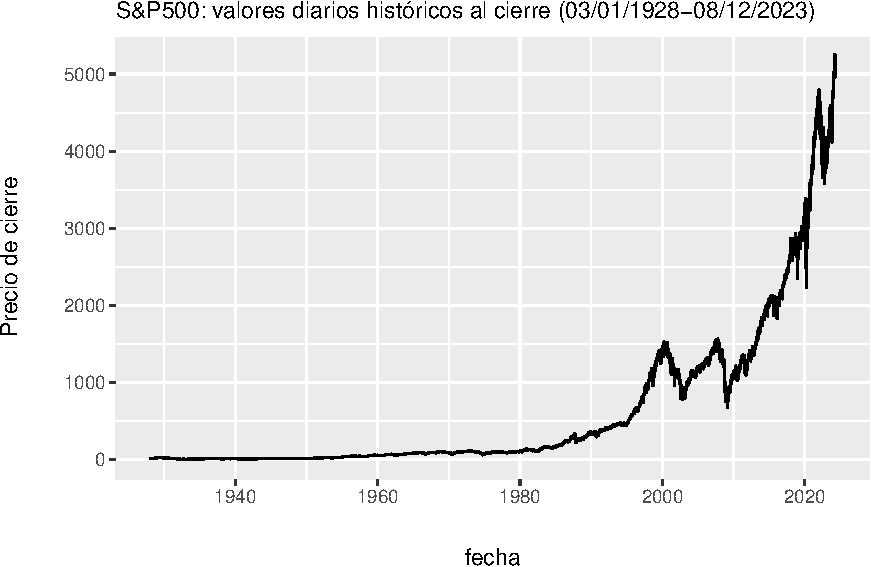
\includegraphics{Entrega_files/figure-latex/unnamed-chunk-21-1.pdf}

\newpage

En la siguiente figura se muestra la evolución del indicador \(IVP\)
relativo a \(S\&P\; 500\) desde la fecha 03/01/1928 hasta 08/12/2023.
\vspace{1cm}

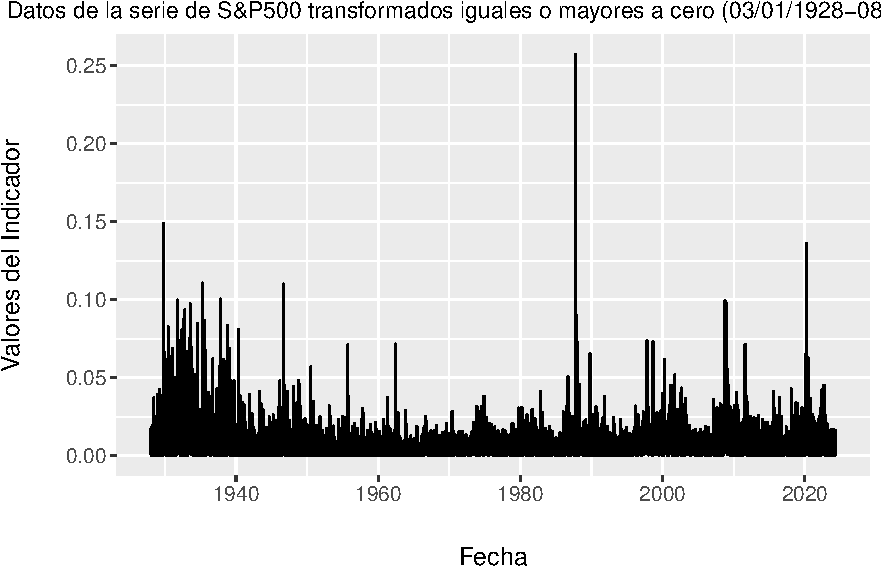
\includegraphics{Entrega_files/figure-latex/unnamed-chunk-22-1.pdf}

\newpage

\section{Marco teórico}\label{marco-teuxf3rico}

\subsection{La teoría asintótica clásica, las distribuciones extremales
y sus dominios de
atracción}\label{la-teoruxeda-asintuxf3tica-cluxe1sica-las-distribuciones-extremales-y-sus-dominios-de-atracciuxf3n}

Como introducción, se presenta de manera sintética la teoría clásica
relacionada a la estadística de eventos extremos que sirve de sustento
para entender el método Peaks over threshold (POT) de la próxima
sección. Para esto, se parte de suponer que \(X\) e \(Y\) son variables
aleatorias \(i.i.d\) con distribuciones son \(F\) y \(G\),
respectivamente. Entonces, la variable

\begin{equation}
max(X,Y)
\end{equation}

tiene por distribución la función \(H\) definida por

\begin{equation}
H(t)= F(t) G(t)
\end{equation}

Por lo tanto, si se tiene datos \(X_1,...,X_n\) \(i.i.d\) con
distribución \(F\) se puede expresar

\begin{equation}
X_n^* = max (X_1,...,X_n)
\end{equation}

con distribución \(F_n^*\) dada por

\begin{equation}
F_n^* (t)= F(t)^n
\end{equation}

Como no es viable\footnote{O manejable} para todos los casos conocer la
distribución \(F\) y la de \(F_n^*\), en una línea de trabajo similar a
la que aporta el Teorema Central del Límite en la estadística de valores
medios, se emplea un teorema para aproximar \(F_n^{*}\) con
distribuciones más sencillas: el Teorema de Fischer-Tippet-Gnedenko
(FTG).

\begin{mydefinition}
Como $X_1,...,X_n$ se supone $i.i.d$, si definimos 
$Y_i = -X_i$ para todo valor de $i$, entonces $Y_1,...,Y_n$ es $i.i.d$ y
además
\begin{equation}
min(X_1,...,X_n) = - max(Y_1,...,Y_n)
\end{equation}
\end{mydefinition}

La teoría asintótica de los mínimos de datos \(i.i.d\) se reduce a la de
los máximos, razón por la que se concentra el estudio en el
comportamiento asintótico de los máximos exclusivamente.

\begin{mydefinition}
 Existen tres tipos de distribuciones extremales: Gumbel, Weibull y Fréchet. En su versión estándar\footnote{También llamada típica.}, una variable se puede distribuir de las siguientes maneras:

\begin{itemize}
\item Gumbel si su distribución es 

\begin{equation}
\Lambda(x) = exp\{-e^{-x}\} \quad\text{para todo}\; x \;\text{real} 
\end{equation}

\item Weibull de orden $\alpha>0$ si su distribución es

\begin{equation}
\Psi_{\alpha}(x)=\begin{cases}
exp\{-(-x)^{\alpha}\} & si\;x<0\\
1 & \text{en otro caso}
\end{cases}
\end{equation}

\item Fréchet de orden $\alpha>0$ si su distribución es

\begin{equation}
\Phi_{\alpha}(x)=\begin{cases}
exp\{-x^{-\alpha}\} & si\;x>0\\
0 & \text{en otro caso}
\end{cases}
\end{equation}
\end{itemize}
\end{mydefinition}

\paragraph*{Nota:}

Como los máximos en general son valores grandes, importa particularmente
observar el comportamiento de estas distribuciones para \(x\) tendiendo
a infinito. El límite es 1 como en toda distribución. Sin embargo,
tiende más rápido a 1 cuando es Weibull, luego Gumbel y por último la
distribución Fréchet. Lo anterior indicaría que la Fréchet modela datos
considerados ``más extremos'', es decir, máximos de datos de colas más
pesadas que la Gumbel y, a su vez, más que la
Weibull\footnote{En la distribución Fréchet, la velocidad de convergencia a 1 crece al aumentar el orden. En cambio en la distribución Weibull el orden afecta la velocidad con que tiende a 0 cuando $x$ tiende a menos infinito, que a su vez, crece cuanto mayor el orden.}.

A las mencionadas distribuciones típicas se las puede extender agregando
un parámetro de recentramiento (\(\mu\)) y un parámetro de escala
(\(\beta\)):

\begin{itemize}
\item Gumbel: se dice que $X$ tiene distribución $\Lambda^{(\mu,\beta)}$ si
\begin{equation}
X=\mu+\beta Y,
\end{equation}
donde $Y$ tiene distribución $\Lambda$.

\item Weibull: se dice que $X$ tiene distribución $\Psi_{\alpha}^{(\mu,\beta)}$ si 
\begin{equation}
X=\mu+\beta Y,
\end{equation}
donde $Y$ tiene distribución $\Psi_{\alpha}$.

\item  Fréchet: se dice que $X$ tiene distribución $\Phi_{\alpha}^{(\mu,\beta)}$ 
\begin{equation}
X=\mu+\beta Y
\end{equation}
donde $Y$ tiene distribución $\Phi_{\alpha}$
\end{itemize}

En general se emplean las distribuciones con los parámetros de
recentramiento y reescalamiento a no ser que no sean relevantes.

\begin{theorem} Relaciones entre las versiones standard de las distribuciones extremales

$$
X\text{ se distribuye }\:\Phi_{\alpha}(x) \iff -\frac{1}{X}\text{ se distribuye }\:\Psi_{\alpha}(x) \iff log(X^{\alpha})\text{ se distribuye }\:\Lambda
$$
\end{theorem}

\paragraph*{Observación 5}

La función Gamma (\(\Gamma\)), que extiende la función factorial
\(\Gamma(n)=n-1!\) para todo \(n\) natural, se define como

\begin{equation}
\Gamma(u)=\int_0^{\infty}t^{u-1}e^{-t}dt
\end{equation}

\begin{theorem}
(Tres en uno) Algunos datos de las distribuciones extremales.
\begin{itemize}
\item Parte 1: si $X$ tiene distribución $\Lambda^{(\mu,\beta)}$ entonces tiene que
\begin{itemize}
  \item[a)] Valor esperado: $E(X) = \mu + \beta\gamma$, donde $\gamma$ es la constante de Euler-Mascheroni, cuyo valor aproximado es $0.5772156649$.
  \item[b)] Moda: $\mu$
  \item[c)] Mediana: $\mu - \beta \log(\log 2) \approx \mu - 0.36651 \beta$.
  \item[d)] Desviación estándar: $\beta \pi \sqrt{6} \approx 1.2825 \beta$.
  \item[e)] Si $X^+ = \max(X,0)$, entonces $E(X^{+k})$ es finito para todo valor de $k$ natural.
  \item[f)] Para simular computacionalmente $X$, se puede tomar $U$ uniforme en $(0,1)$ y  calcular $$X = \mu - \beta \log(-\log U)$$.
\end{itemize}
\item Parte 2: si $X$ tiene distribución $\Psi_{\alpha}^{(\mu,\beta)}$ entonces tiene que
\begin{itemize}
  \item[a)] Valor esperado: $E(X) = \mu + \beta\Gamma(1+1/\alpha)$.
  \item[b)] Moda: $\mu$ si $\alpha\leq 1$ y $\mu-\beta\{(\alpha-1)/\alpha\}^{(1/\alpha)}$ si $\alpha>1$.
  \item[c)] Mediana: $\mu - \beta \log(2)^{(1/\alpha)}$.
  \item[d)] Desviación estándar: $\beta\{\Gamma(1+2/\alpha)-\Gamma(1+1/\alpha)^2\}^{1/2}$.
\end{itemize}
\item Parte 3: si $X$ tiene una distribución $\Phi_{\alpha}^{(\mu, \beta)}$ entonces se tiene que
\begin{itemize}
  \item[a)] Valor esperado: $E(X) = \mu + \beta\Gamma(1-1/\alpha)$ si $\alpha > 1$, $\infty$ en caso contrario.
  \item[b)] Moda: $\mu + \beta\Gamma(1-1/\alpha)$ si $\alpha>1$.
  \item[c)] Mediana: $\mu + \beta \log(2)^{(-1/\alpha)}$.
  \item[d)] Desviación estándar: $\beta|\Gamma(1-2/\alpha)-\Gamma(1-1/\alpha)^2|$ si $\alpha>2$, $\infty$ si $1<\alpha \leq 2$.
\end{itemize}
\end{itemize}
\end{theorem}

\paragraph*{Observación 6}

El item e) de la Parte 1 es trivialmente cierto para Weibull y, tomando
en cuenta el item a) de la Parte 3, es falso para Fréchet.

\paragraph*{Observación 7}

El item f) de la Parte 1 en conjunto con el Teorema 1 provee de fórmulas
sencillas para simular computacionalmente distribuciones Weibull o
Fréchet.

\begin{theorem} Fischer-Tippet-Gnedenko (FTG)

Si $X_1,...,X_n\quad .i.i.d$ con distribución $F$ "continua"\footnote{Cabe resaltar que la continuidad de la distribución $F$ no es una hipótesis real (ni es necesaria ni es suficiente), pero ayuda a visualizar que no vale el teorema para toda distribución $F$.}, llamamos $F_n^*$ a la distribución de $max(X_1,...,X_n)$ y $n$ es grande, entonces existen $\mu$ real y $\beta>0$ tales que alguna de las siguientes tres afirmaciones es correcta:

\begin{itemize}
  \item[1)] $F_n^*$ se puede apromixar por la distribución de $\mu+\beta Y$ con $Y$ variable con distribución $\Lambda$.
  \item[2)] Existe $\alpha>0$ tal que $F_n^*$ se puede aproximar por la distribución de $\mu+\beta Y$ con $Y$ variable con distribución $\Phi_{\alpha}$. 
  \item[3)] Existe $\alpha>0$ tal que $F_n^*$ se puede aproximar por la distribución de $\mu+\beta Y$ con $Y$ variable con distribución $\Phi_{\alpha}$.
\end{itemize}
\end{theorem}

Lo anterior equivale a decir que la distribución del máximo de datos
\textit{continuos} e \(iid\), si \(n\) es grande, puede aproximarse por
una Gumbel, una Fréchet o una Weibull.

La distribución \(F\) determina la apromicación a tomar:

\begin{itemize}
\item Cuando $F$ sea normal entonces $F_n^*$ se puede aproximar como una Gumbel
\item Cuando $F$ sea uniforme, se puede aproximar $F_n^*$ como una Weibull
\item Cuando $F$ sea Cauchy entonces $F_n^*$ se puede aproximar por una Fréchet
\end{itemize}

Más precisamente, cuál de las tres aproximaciones es la aplicable
depende de la cola de \(F\) (los valores de \(F(t)\) para valores
grandes de \(t\)).

En concreto, Weibull aparece cuando \(F\) es la distribución de una
variable acotada por arriba (como la Uniforme), Gumbel para
distribuciones de variables no acotadas por arriba pero con colas muy
livianas (caso Exponencial y Normal) y Fréchet para colas pesadas (caso
Cauchy)\footnote{Si bien  la hipótesis de continuidad de $F$ no es esencial, si $F$ tiene
la distribución Binomial o Poisson, por ejemplo, no se puede aplicar ninguna de las tres aproximaciones anteriores.}.

\paragraph*{Observación 10}

Como consecuencia del FTG, si se tienen datos de máximos, las
distribuciones extremales son ``candidatas'' razonables para proponer en
un ajuste. Sin embargo, no siempre se va a lograr ajustar una de las
tres distribuciones extremales, ya que hay al menos dos causas que
podrían desafiar la aplicación del FTG:

\begin{itemize}
\item Cuando la cantidad de registros no es lo suficientemente grande
\item Cuando los registros que se consideran al calcular cada máximo no sean $i.i.d$\footnote{Sin embargo, esto puede subsanarse con versiones más generales del FTG.}
\end{itemize}

Entonces, aunque el FTG alienta a intentar ajustar datos extremales a
una de las tres distribuciones extremales, pero no siempre un tal ajuste
dará un resultado afirmativo.

Como la mayoría de pruebas de ajuste suponen datos \(iid\), se van a
realizar dos tests de
aleatoriedad\footnote{En inglés se expresa como \textit{randomness}} a
los datos (\textit{runs up and down} y
\textit{pearman correlation of ranks}).

Se emplea la prueba de ajuste \(\chi^2\) que requiere seleccionar una
partición más o menos arbitraria de la recta real de intervalos siendo
importante que en cada intervalo haya una cantidad lo suficientemente
importante de datos de la muestra. En este sentido, se pueden tomar como
extremos de los intervalos los quintiles empíricos de la muestra. Cabe
mencionar que este test requiere estimar parámetros por el método de
Máxima Verosimilitud Categórica, que da resultado distintos al método de
Máxima Verosimilitud a secas
\footnote{Este hecho es frecuentemente ignorado y presentado erróneamente en los textos y cursos básicos de Estadística, ya que da resultados distintos al método de Máxima Verosimilitud a secas. Este hecho es frecuentemente ignorado y presentado erróneamente en los textos y cursos básicos de Estadística.}.

\begin{definition} Distribución Extremal Asintótica (DEA)

Si $X_1,...,X_n$  es $iid$ con distribución $F$ diremos que $H$ no-degenerada\footnote{Cabe mencionar que para este estudio la distribución de la variable a incorporar no tiene que ser degenerada, es decir $H(t)=0$ ó $H(t)=1$. Una distribución $H$ se dice degenerada si $H(t)=0$ ó $1$ para todo valor de $t$. Si la distribución de $X$ es degenerada, entonces $X$ es una constante, y no tiene sentido hacer estadística sobre $X$, por lo tanto sólo tienen interés las distribuciones no-degeneradas.} es la Distribución Extremal Asintótica (DEA) de $F$\footnote{Lo que equivale a decir que $F$ tiene $DEA\;H$.}, si existen dos sucesiones de números reales, $d_n$ y $c_n>0$, tales que la distribución de

\begin{equation}
\frac{max(X_1,...,X_n)- d_n}{c_n}\label{eq:max}
\end{equation}

tiende a $H$ cuando $n$ tiende a infinito.
\end{definition}

\begin{definition} Supremo esencial de una variable aleatoria o distribución

Si $X$ tiene distribución $F$, se llama supremo esencial de $X$, denotado como $M_X$ o, indistintamente, supremo esencial de $F$ denotado $M_F$ a

\begin{equation}
M_X=M_F= sup\{t / F(t)<1\}\label{eq:Mx}
\end{equation}
\end{definition}

\paragraph*{Observación 11}

\begin{itemize}
\item Si $F$ es $U(a,b) \Rightarrow M_F=b$
\item Si $F$ es $Bin(m,p) \Rightarrow M_F=m$
\item Si $F$ es Normal, Exponencial, Cauchy o Poisson, $M_F$ es infinito.
\end{itemize}

\begin{theorem} 
Si $X_1,...,X_n$ es $iid$ con distribución $F$ cualquiera, entonces, para $n\longrightarrow \infty$,
\begin{equation}
X^*_n=M_F= max(X_1,...,X_n)\;\longrightarrow\;M_F \label{eq:Xast}
\end{equation}
\end{theorem}

\paragraph*{Observación 12}

El resultado anterior vale incluso si \(M_F\) es infinito, pero si
\(M_F\) es finito, como \(X^*n - M_F\) tiende a cero, por analogía con
el Teorema Central del Límite para promedios, buscaríamos una sucesión
\(c_n>0\) y que tienda a cero de modo tal que \((X^*n- M_F )/ c_n\)
tienda a una distribución no-degenerada y de allí surge buscar la DEA.

\begin{theorem}
Si $F$ es una distribución con $M_F$ finito, y para $X$ con distribución $F$ se cumple que
$$
P(X=M_F)>0 
$$
entonces $F$ NO admite DEA\footnote{Este teorema brinda una condición NECESARIA pero NO SUFICIENTE para DEA}.
\end{theorem}

\paragraph*{Observación 13}

Si \(F\) es \(Bin(m,p)\), \(M_F=m\). Si \(X\) tiene distribución \(F\),
entonces \(P( X=M_F)= P( X=m)= p_m>0\), asi que la distribucion
\(Bin(m,p)\) NO admite DEA, no se puede aproximar la distribución del
máximo de una muestra \(iid\) de variables \(Bin(m,p)\).

El Teorema anterior es un caso particular del próximo.

\begin{theorem}
Si $F$ es una distribución con $M_F$ finito o infinito que admite DEA, y $X$ tiene distribución $F$, entonces el límite cuando $t$ tiende a $M_F$ por izquierda de
$$P(X>t)/P(X \geq t)$$
debe ser 1.
\end{theorem}

\paragraph*{Observación 14}
\begin{itemize}
\item Si $F$ es una distribución de Poisson de parámetro $\lambda>0$, $M_F$ es infinito. 
\item Si $k$ es un natural, entonces:
\begin{eqnarray}
\frac{P(X>k)}{P(X\geq k)} &=& \frac{P(X \geq k+1)}{P(X\geq k)} \\ \nonumber
&=& 1-\frac{P(X=k)}{P(X \geq k)} \approx 1-\left(1- \frac{\lambda}{k}\right) 
\end{eqnarray}
que tiende a $0$ cuando $k$ tiende a infinito, por lo cual $F$ NO admite DEA, o sea que no se puede aproximar el máximo de una sucesión $iid$ de variables de Poisson.
\end{itemize}

Algunos ejemplos donde la DEA resulta aplicable:

\paragraph*{Observación 15}

Si \(F\) es \(U(0,1)\) y consideramos \(X_1,...,X_n\) \(iid\) con
distribución \(F\), resulta que la distribución de \(n( X_n^*- 1)\)
tiende a \(\Psi_1\) por lo cual la distribución uniforme tiene DEA
Weibull.

\paragraph*{Observación 16}

Si \(F\) es Exponencial de parámetro 1 y consideramos \(X_1,...,X_n\)
\(iid\) con distribución \(F\), se tiene que la distribución de
\(X_n^*- log\: n\) tiende a \(\Lambda\) por lo cual la distribución
exponencial tiene DEA Gumbel.

\paragraph*{Observación 17}

Si F es \(N(0,1)\) y consideramos \(X_1,...,X_n\) \(iid\) con
distribución \(F\), definimos la función continua y estrictamente
decreciente (para \(u>0\))

\[
g(u)=e^{(-u^2/4\pi)/u}
\]

que \(g(u)\rightarrow \infty\) cuando \(u\rightarrow 0\), y
\(g(u)\rightarrow 0\) cuando \(u\rightarrow \infty\). Por lo cual para
todo natural \(n\) existe un único valor \(u_n\) tal que

\[
g(u_n)=1/n
\]

y resulta que
\(\frac{u_n}{\sqrt{2\pi}\left (X_n^*-\frac{u_n}{\sqrt{2\pi}}\right )}\longrightarrow \Lambda\)
por lo que la distribución normal tiene DEA Gumbel.

\paragraph*{Observación 18}

Si \(F\) es Cauchy standard tal que \(C(0,1)\) y consideramos
\(X_1,...,X_n\) \(i.i.d\) con distribución \(F\), se tiene que la
distribución de \(\pi X^*_n/n\) tiende a \(\Phi_1\), por lo cual la
distribución Cauchy tiene DEA Fréchet.

Cuando \(F\) admite DEA, la distribución \(H\) deberá ser una
distribución extremal. De hecho FTG resulta de combinar dos teoremas,
basadas en una nueva definición, la de distribución max-estable.

\begin{definition} Distribución max-estables

Si dado $F$ representando una distribución, $X$ con distribución $F$, $k$ natural arbitrario y $X_1,...,X_k$ es $iid$ con distribución $F$, existen reales $a_k$, $b_k$ tales que $max(X_1,...,X_k)$ tiene la misma distribución que $a_k X+ b_k$, $F$ se dice \textit{max-estable}.
\end{definition}

El Teorema FTG resulta de superponer los dos siguientes teoremas:

\begin{theorem} 
\begin{itemize}
  \item[a)] Si $F$ admite $DEA\;H$, entonces $H$ es max-estable.
  \item[b)] Si $H$ es max-estable, es la DEA de sí misma.
\end{itemize}
\end{theorem}

\begin{theorem}
Una distribución es max-estable si y solo si es extremal\footnote{O sea Gumbel, Weibull o Fréchet}.
\end{theorem}

\paragraph*{Observación 19}

Si \(F\) y \(G\) son dos distribuciones, tienen colas equivalentes si
\(M_F=M_G\) y cuando \(t\) tiende a \(M_F\) por izquierda,
\((1-F(t))/(1-G(t))\) tiende a un valor \(c>0\).

La distribución del máximo de dos variables independientes se calcula
como \(max\{X,Y\}\), cuando \(X\) e \(Y\) son independientes y cada una
de ellas es una distribución extremal, se llega al siguiente resultado:

\begin{longtable}[]{@{}
  >{\raggedright\arraybackslash}p{(\columnwidth - 4\tabcolsep) * \real{0.2500}}
  >{\raggedright\arraybackslash}p{(\columnwidth - 4\tabcolsep) * \real{0.2500}}
  >{\raggedright\arraybackslash}p{(\columnwidth - 4\tabcolsep) * \real{0.5000}}@{}}
\toprule\noalign{}
\begin{minipage}[b]{\linewidth}\raggedright
\(X\)
\end{minipage} & \begin{minipage}[b]{\linewidth}\raggedright
\(Y\)
\end{minipage} & \begin{minipage}[b]{\linewidth}\raggedright
\(max(X,Y)\)
\end{minipage} \\
\midrule\noalign{}
\endhead
\bottomrule\noalign{}
\endlastfoot
\textcolor{red}{Weibull} & \textcolor{red}{Weibull} &
\textcolor{red}{Weibull} \\
\textcolor[rgb]{0.0,0.5,0.0}{Weibull} &
\textcolor[rgb]{0.0,0.5,0.0}{Gumbel} &
\textcolor[rgb]{0.0,0.5,0.0}{Cola equivalente Gumbel} \\
\textcolor{blue}{Weibull} & \textcolor{blue}{Fréchet} &
\textcolor{blue}{Fréchet} \\
\textcolor[rgb]{0.0,0.5,0.0}{Gumbel} &
\textcolor[rgb]{0.0,0.5,0.0}{Weibull} &
\textcolor[rgb]{0.0,0.5,0.0}{Cola equivalente Gumbel} \\
\textcolor{red}{Gumbel} & \textcolor{red}{Gumbel} &
\textcolor{red}{Gumbel} \\
\textcolor{blue}{Gumbel} & \textcolor{blue}{Fréchet} &
\textcolor{blue}{Cola equivalente Fréchet} \\
\textcolor{blue}{Fréchet} & \textcolor{blue}{Weibull} &
\textcolor{blue}{Fréchet} \\
\textcolor{blue}{Fréchet} & \textcolor{blue}{Gumbel} &
\textcolor{blue}{Cola equivalente Fréchet} \\
\textcolor{red}{Fréchet} & \textcolor{red}{Fréchet} &
\textcolor{red}{Fréchet} \\
\end{longtable}

\textcolor{red}{\rule{1em}{1em} Las extremales son max-estables: tomar máximos de dos del mismo tipo queda en el mismo tipo.}

\textcolor[rgb]{0.0,0.5,0.0}{\rule{1em}{1em} Gumbel es más pesada que Weibull. En la cola, que es lo que cuenta para máximos, prima Gumbel.}

\textcolor{blue}{\rule{1em}{1em} Fréchet es más pesada que Gumbel y mucho más pesada que Weibull.}
\vspace{1cm}

Además, de la tabla se deduce que

\begin{theorem}
Si $X_1,...,X_n$ independientes y cada $X_i$ tiene uno de los tres tipos de distribución extremal, entonces la distribución del $max(X_1,...,X_n)$ es:
\begin{itemize}
\item[a)] Cola equivalente a Fréchet, si alguna de las variables es Fréchet y alguna otra es Gumbel.
\item[b)]  Fréchet, si alguna es Fréchet y ninguna es Gumbel.
\item[c)]  Cola equivalente Gumbel ninguna es Fréchet pero algunas son Gumbel y otras Weibull.
\item[d)] Gumbel si todas son Gumbel.
\item[e)]  Weibull si todas son Weibull.
\end{itemize}
\end{theorem}

\subsubsection*{Dominio de Atracción Maximal}

\paragraph*{Observación 20}

Si \(F\) es una distribución, se dice que tiene cola de variación
regular de orden \(-\alpha\), para \(\alpha \geq 0\) si, para todo
\(t>0\), \((1-F(tx))/(1-F(x))\) tiende a \(t^{-\alpha}\) si
\(x \rightarrow \infty\). Para abreviar se dirá que \(F\) es
\(R_{-\alpha}\). Por ejemplo, para \(\alpha=3\) un caso de una tal \(F\)
es \(F(u)=1- 1/u^3\).

Por otra parte se dice que \(L\) es una función de variación lenta si,
para todo \(t>0\), \(L(tx)/L(x)\) tiende a 1 cuando
\(x \rightarrow \infty\). Un ejemplo es \(L(u)=log(u)\).

\begin{definition} Dominio de Atracción Maximal ($DAM$)

Si $H$ es una distribución extremal (Gumbel, Weibull o Fréchet) su Dominio de Atracción Maximal ($DAM(H)$), está constituído por todas las distribuciones $F$ que tienen DEA $H$.
\end{definition}

\begin{theorem} DAM de la Fréchet

$F$ pertenece a la $DAM$ de $\Phi_{\alpha}$ si y sólo si
$1-F(x)=x^{-\alpha} L(x)$ para alguna $L$ de variación lenta,
lo cual es equivalente a decir que $F$ es $R_{-\alpha}$. Un ejemplo típico sería $1-F(x)= x^{-\alpha}$.

Además, puede tomarse $d_n=0$ y $c_n= n^{1/\alpha}$.
\end{theorem}

\begin{Corolario} DAM de la Fréchet

Si $F$ es una distribución con densidad $f$ que cumple que $xf(x)/(1-F(x))$ tiende a $\alpha$ cuando $x\rightarrow \infty$ se dice que $F$ cumple la Condición de Von Mises I. En tal caso, $F$ pertenece a la DAM de $\Phi_{\alpha}$ y más aún, la DAM de $\Phi_{\alpha}$ son todas las distribuciones que tienen cola equivalente a alguna distribución que cumpla la Condición de Von Mises I.
\end{Corolario}

Del DAM Fréchet y Teorema 1, surge lo siguiente.

\begin{theorem} DAM de la Weibull

\begin{itemize}
\item[a)] $F$ pertenece a la DAM de $\Psi_{\alpha}$ si y sólo si $M_F$ es finito y además $1-F(M_F -1/x)=x^{-\alpha}L(x)$ para alguna $L$ de variación lenta, es decir que pertenece a $R_{-\alpha}$. Observar que con el cambio de variable $u=M_F -1/x$,
resulta que $1-F(u)=(^{-}M_F -u)^{\alpha} L(1/(M_F -u))$ para alguna $L$ de variación lenta, para $u< M_F$. Un ejemplo típico sería $1-F(u)=(^{-}MF -u)^{\alpha}$ , $u< M_F$. 

Además puede tomarse $d_n= M_F$ y $c_n= n^{-\alpha}$.

\item[b)] Si $F$ es una distribución con densidad $f$ positiva en $(a,M_F)$ para algun $a< M_F$ y $(M_F -x)f(x)/(1-F(x))$ tiende a $\alpha$ cuando $x\rightarrow M_F$, se dice que $F$ cumple la Condición de Von Mises II. En tal caso $F$ pertenece a la DAM de $\Psi_{\alpha}$ y mas aún,la DAM de $\Psi_{\alpha}$ son todas las distribuciones que tienen cola equivalente a alguna distribución que cumpla la Condición de Von Mises II.
\end{itemize}
\end{theorem}

\begin{theorem} DAM de la Gumbel

Una distribución $F$ se dice una Función de Von Mises con función auxiliar $h$ si existe $a < M_F$ ($M_F$ puede ser finito o infinito) tal que para algún $c>0$ se tiene

$$
1-F(x)=c\:exp\left \{  - \int_a^x \frac{1}{h(t)} dt \right \}
$$

con $h$ positiva, con densidad $h^{\prime}$ y $h^{\prime}(x)$ tendiendo a $0$ para $x \rightarrow M_F$.
\end{theorem}

\begin{Corolario}
Si $F$ pertenece al DAM Gumbel , $M_F$ es infinito, y se considera $X$ con distribucion $F$, entonces $E(X^{+k})$ es finito para todo $k$ natural.
\end{Corolario}

A modo de conclusión, los resultados antes vistos nos permiten reconocer
que distribuciones tienen DEA y si la tienen, cual es. Adicionalmente,
permiten entender que esta teoría se relaciona con el comportamiento de
las colas de las distribuciones, esto es, que Fréchet corresponde a las
colas más pesadas, luego la Gumbel y finalmente Weibull.

\newpage

\subsubsection*{GEV: Distribución de valores extremos generalizada}

La GEV permite compactar en una única fórmula las tres distribuciones
extremales.

\begin{definition} GEV

Se define la distribución de valores extremos generalizada (GEV) por sus siglas en ingles de posición $\mu$, escala $\beta$ e índice $\xi$ a

\begin{align*}
G(\mu, \beta, \xi) = \begin{cases}
e^{ -\left ( 1+\xi(t-\mu)/\beta \right )^{-1/\xi} } & \text{si } \xi\neq 0\; \forall t \text{ donde } 1+\xi(t-\mu)/\beta>0\\ 
e^{ -e^{\left ( -(t-\mu)/\beta \right )}} & \text{si } \xi=0 \; \forall t
\end{cases}
\end{align*}
\end{definition}

El caso \(\xi=0\) corresponde a Gumbel, el caso \(\xi<0\) a Weibull y
\(\alpha=-1/ \xi\), el caso \(\xi>0\) a Fréchet y
\(\alpha=1/ \xi\)\footnote{En \texttt{R} existen rutinas para estimar $\xi$ con intervalos de confianza (por máxima verosimilitud, etc.) lo cual da formas de testear si una extremal es Gumbel, Weibull o Fréchet.}.

\subsubsection*{Tiempos y Valores de Retorno}

En Ingeniería y Ciencias Ambientales, suele pensarse los eventos
extremos, en términos de tiempos de retorno, o sea, el tiempo que se
espera para que ocurra un evento. Bajo las hipótesis de datos \(iid\),
el tiempo de retorno \(T\) tiene una distribución \(Geo(p)\), con
\(p = P(evento)\), por lo cual el tiempo de retorno medio es
\(E(T)=1/p\). Pueden hacerse intervalos de confianza para \(E(T)\), en
la medida que exista información de \(P(evento)\). Cabe observar que
muchas veces se utiliza la expresión Tiempo de Retorno (TR) para
\(E(T)\).

Más precisamente, \(TR(u)\), el Tiempo de retorno del valor \(u\), es el
valor esperado (o la media) del tiempo que se debe esperar para que la
variable en estudio supere el valor \(u\), es decir que
\(TR(u) = 1/P(X>u)\), si \(X\) es la variable en estudio.

Por otro la lado, en una mirada inversa, el Valor de Retorno a tiempo
\(t\), \(VR(t)\) es el valor de \(u\) para el cual \(TR(u)=t\), es decir
que \(TR(VR(t))=t\) (y también \(VR(TR(u))=u\), por lo que \(TR\) y
\(VR\) serían funciones inversas).

\subsection{Un primer enfoque de datos no
iid}\label{un-primer-enfoque-de-datos-no-iid}

En la realidad, frecuentemente, los datos no son \(iid\). En la teoría
de series de tiempo, se suele expresar la expresión ``Ruido Blanco''
para referirse a datos iid. Se caracterizan por tener espectro
constante.

Si los datos no necesariamente son independientes pero la estructura de
distribuciones es siempre la misma, se habla de datos estacionarios (o
procesos estacionarios). Siguiendo a Enders
(\citeproc{ref-enders}{2014}), se dice que un proceso estocástico
\(z_{t}\) con media y varianza finitas es estacionario en covarianza
para todo \(t\) y \(t-s\) cuando

\begin{align}
    \label{eq:2_7}
    E(z_{t})&=E(z_{t-s})=\mu\\
    \label{2_8}
    var(z_t)&=var(z_{t-s})=\sigma^2_z\\
    \label{2_9}
    cov(z_t,z_{t-s})&=cov(z_{t-j},z_{t-j-s})=\gamma_s
\end{align} donde \(\mu, \sigma^2_z, \gamma_s\) con constantes.

En \(var(z_t)=var(z_{t-s})=\sigma^2_z\), cuando \(s=0\) se va a tener
que \(\gamma_0\) es la varianza de \(z_t\). Que una serie temporal sea
estacionaria en covarianza implica que tanto la media como todas sus
autocovarianzas\footnote{También se habla de proceso debilmente estacionario o estacionario de segundo orden.}
no están afectadas por cambios en los orígenes temporales.

Cuando los datos no son independientes pero la dependencia se va
atenuando a medida que se consideran datos más lejanos (para fijar
ideas, imaginemos que los datos corresponde a medidas en el tiempo, y
que datos muy viejos no influirían significativamente sobre el presente,
por ejemplo), se habla de datos débilmente dependientes. El caso más
sencillo de esta situación es la de datos \(m-\)dependientes (donde
\(m\) es un número), que corresponde a datos que si están a distancia
mayor a \(m\), son independientes. Es el caso de los procesos \(MA(q)\)
( Moving Averages), que son Promedios Móviles de orden \(q\) de un ruido
blanco (\(m=q\) en este caso).

Los procesos \(AR(p)\) (Autoregresivos de orden \(p\)) son débilmente
dependientes pero no \(m\)-dependientes para ningún \(m\); cada dato es
una combinación lineal de los \(p\) anteriores más un término aleatorio
(``Ruido'') que es un ruido blanco. Son Markovianos, es decir, con
memoria infinita pero donde todo el pasado es tan informativo como los
últimos \(p\) datos.

En la teoría clásica de series de tiempo, una estructura AR(p) a partir
de un ruido MA(q) en lugar de un ruido blanco, da lugar a los procesos
ARMA (p,q), que en general son débilmente dependientes y aproximan bien
a cualquier proceso estacionario débilmente dependiente, lo cual es una
de las razones de su popularidad. Lo opuesto a dependencia débil es
dependencia fuerte.

Cuando los datos no son \(iid\) pero se vuelven \(iid\) al restarle una
función determinística, son bastante simples de manejar. Si esta función
es monótona, se habla de que los datos presentan tendencias (trends). Si
en cambio la función es periódica, se dice que los datos presentan
ciclos (seasonal effects). Se puede demostrar que si los datos se
vuelven \(iid\) al restar una función determinística cualquiera (lo cual
no siempre es el caso!), entonces se pueden modelar aproximadamente como

\[
TENDENCIAS+CICLOS+ DATOS IID.
\] Si se le restara a los datos originales los valores de las
componentes determinísticas (Tendencia+Ciclo) ajustadas, los nuevos
datos que resultan (llamados Residuos) deberían razonablemente superar
los tests para datos iid.

Como resumen final, en los más próximos capítulos tomaremos direcciones
no iid, en las que veremos: 1.Si el proceso es estacionario y débilmente
dependiente, la técnica clásica de DEA puede aplicarse esencialmente
igual (Leadbetter, Lindgren, Rootzén). 2.Si el proceso no es
estacionario o no es débilmente dependiente, cumple algunas propiedades
condicionales a otro proceso que le pauta la ``fase'', la técnica
clásica de DEA puede aplicarse, pero con modificaciones no menores.

Además: 3.Puede cambiarse el enfoque y mirar el número de eventos
extremos en diversos lapsos, esto lleva en el caso iid a un proceso de
Poisson, para estacionarios y débilmente dependientes a un Poisson
Compuesto y en el marco más general del punto 2, a mezclas de Procesos
de Poisson Compuestos ( Lise Bellanger-GP). El conteo de eventos
extremos será también la base o el ``pie'', para introducir una técnica
muy usada, POT (Picos Sobre Umbrales) y sus variaciones más recientes
que veremos al final.

\newpage

\subsection{Peaks Over Treshold (POT) y
variantes}\label{peaks-over-treshold-pot-y-variantes}

Vamos ahora a volver a cambiar el enfoque de manera importante. Como en
el capítulo anterior, fijaremos un cierto umbral, llamaremos
\emph{evento} cuando la variable observada supera ese umbral, nos
concentraremos en los eventos, pero, a diferencia del capítulo anterior,
no nos quedaremos con el conteo de eventos, sino que no sinteresa ver
cómo se comporta el ``exceso'' de nuestro registro. De este modo
pretendemos obtener información más fina que con HLE o con DEA, ya que
no miramos como se distribuye el valor más grande registrado sino que
pretendemos ver cómo se distribuyen los valores muy elevados (por encima
del umbral).

Dicho de otra manera, si \(u\) es el umbral y \(X\) es nuestro registro,
cuando \(X>u\) tendremos un \emph{evento} y queremos estudiar
estadísticamente el \emph{exceso} \(X-u\). Esto es el método POT, que se
apoya en un resultado muy relevante, a menudo referido como Segundo
Teorema de la Teoría Clásica de Valores Extremos (el primero es el FTG).

\begin{definition}[Distribución Pareto Generalizada]
Si $k$ real y $\sigma>0$, la Distribución de Pareto Generalizada $G_{k,\sigma}$ se define de la siguiente manera:\\
\begin{equation}
G_{k,\sigma}(x)=\left\{\begin{matrix}
 1-(1+kx/\sigma)^{-1/k}& si & k\neq 0 \left\{\begin{matrix}
\text{para todo} \;x\geq 0 , & si & k>0\\ 
\text{para todo}\; x \;\text{que cumple}&
0\leq x \leq  -\sigma/k, &si& k<0
\end{matrix}\right.\\ 
 1-e^{(-x/\sigma)} & si& k =0\; \text{para todo}\; x\geq 0
\end{matrix}\right. 
\end{equation}
\end{definition}

\subparagraph{Observación 1}\label{observaciuxf3n-1}

Es obvio a partir de la definición que el caso \(k=0\) corresponde a la
distribución exponencial de parámetro \(1/\sigma\), por lo cual
\(\sigma\) sería la media de la distribución. El caso \(k=-1\)
corresponde a la distribución uniforme en \([0, \sigma]\), or lo cual la
media sería \(\sigma/2\). El caso \(k>0\) corresponde a la distribución
de Pareto.

\subparagraph{Observación 2}\label{observaciuxf3n-2}

Observar que la familia de Distribuciones de Pareto Generalizada es
continua, en el sentido que cuando \(k\) tiende a cero por derecha o
izquierda, \(G_{k,\sigma}\) tiende a \(G_{0,\sigma}\) . Lo mismo ocurre
con las distribuciones extremales vistas en el capítulo 1, como el
lector puede verificar.

\begin{theorem}[de Pickands-Balkema-de Haan $(PBdH)$]
Consideremos una distribución $F$ que admite $DEA$, es decir que pertenece al $DAM$ de alguna distribución extremal. Dado un umbral $u>0$, consideremos la distribución condicional de excesos, definida por
\begin{align}
F_u(x)= &P(X \leq  u+x/ X>u)= \nonumber \\
=&P(u<X \leq u+x)/P(X>u)= \nonumber \\
=&\frac{F(u+x)-F(u)}{1-F(u)}\:\text{para todo}\; x\; en\;(0,M_{F}-u)
\end{align}
\end{theorem}

Entonces, cuando \(u\) tiende a infinito, \(F_u\) tiende tiende a una
Distribución de Pareto Generalizada.

\subparagraph{Observación 3}\label{observaciuxf3n-3}

El método POT para datos \(iid\), se desarrolla así:

\begin{itemize}
\item Paso 1: Se elige “adecuadamente” un umbral grande $u$ (aclararemos este punto más adelante).
\item Paso 2: Se estima $p$, la probabilidad de quedar por debajo del umbral $u$ ($p=F(u)$).
\item Paso 3: Se toma la submuestra constituída únicamente por los datos que superan el umbral $u$.
\item Paso 4: Se verifica que esta submuestra pueda suponerse $iid$, mediante los tests de aleatoriedad (volveremos sobre este punto).
\item Paso 5: Se verifica mediante test de ajuste, que esta submuestra puede modelarse por una Distribución de Pareto Generalizada.
\item Paso 6: Se estiman los parámetros $k$ y $\sigma$. Para abreviar, llamemos $PGE$ a la Pareto Generalizada con los parámetros estimados.
\item Paso 7: Finalmente, si dado $y >u$, se quiere calcular la probabilidad de encontrar un registro que no supere a $y (F(y))$, se calcula como:
\begin{equation}
F(y)=p +(1-p)PGE(y-u)
\end{equation}
\end{itemize}

Aclaremos algunos de los puntos más delicados.

\subparagraph{Observación 4: El ``trade off'' sobre
u}\label{observaciuxf3n-4-el-trade-off-sobre-u}

Es evidente que el Paso 5 se apoya en el Teorema \(PbdH\), por lo cual,
es necesario que \(u\) sea grande. Sin embargo si \(u\) es demasiado
grande, la submuestra del Paso 3 y por ende, al tener pocos datos,
presumiblemente pasará cualquier test que se realice, pero estas
conclusiones serán de muy baja confiabilidad. Y aunque la submuestra
efectivamente sea \(iid\) y se ajuste a una Pareto Generalizada, la
estimación de sus parámetros seguramente sea muy pobre. Por lo tanto,
necesitamos un \(u\) ``grande pero no tanto'', un claro ``trade-off'' al
que referimos con ``adecuadamente'' en el Paso 1. Hay diversas
recomendaciones sobre la elección de \(u\), pero para proponer algo bien
claro y sencillo: proponemos tomar \(u\) grande pero que la submuestra
del Paso 3 tenga al menos una veintena de datos.

\subparagraph{Observación 5: ¿Por qué hacer el Paso
4?}\label{observaciuxf3n-5-por-quuxe9-hacer-el-paso-4}

El motivo para ello es doble. Por un lado, aunque la muestra total haya
pasado tests de aleatoriedad y pueda asumirse \(iid\), podría pasar que
al mirar sólo los valores altos, se detectaran efectos no aleatorios que
hayan pasado desapercibidos en los tests sobre toda la muestra. Por otro
lado, inversamente, puede haber muestras que no sean \(iid\) debido a
efectos no aleatorios que se presenten los valores bajos de la muestra y
que por ende, en los valores altos se observe un comportamiento \(iid\).
Por esta doble razón, recomendamos no obviar el Paso 5.

\subparagraph{\texorpdfstring{Observación 6: El
\emph{clustering}}{Observación 6: El clustering}}\label{observaciuxf3n-6-el-clustering}

En ocasiones, la submuestra del Paso 3 presenta muy claramente
\emph{clustering}, esto es, los pasajes del umbral \(u\) se dan en
``grupitos''. Eso es una pista muy firme que delata la existencia de
dependencia en los datos. Y los datos deben respetarse, siempre. Por lo
tanto en la literatura se encuentran diversas propuestas de
\emph{declustering}, esto es, transformar los \emph{grupitos} en un solo
pasaje.

No somos muy afectos a estos procedimientos (salvo que existan razones
de fondo para considerar que hay reverberaciones o réplicas en las
medidas observadas y maneras sólidamente asentadas de traducirlas en una
única lectura), pues de algún modo se fuerza los datos a adaptarse a un
modelo, en lugar de buscar el mejor modelo para los datos. Por ello,
consideramos más adecuado discutir cómo implementar POT (o variantes) en
datos que presenten dependencia, como se verá más adelante.

Previo a ello, como es usual, veremos un ejemplo de aplicación a datos
concretos, de forma de consolidar los conceptos.

Para ello es necesario establecer algunos conceptos y fórmulas.

\subparagraph{Observación 7: Métodos de
estimación}\label{observaciuxf3n-7-muxe9todos-de-estimaciuxf3n}

El método de estimación de parámetros por Máxima Verosimilitud es muy
simple en el caso \(iid\), pero más complejo en otros contextos. Sin
embargo, desde el momento que los métodos basados en momentos y en
cuantiles funcionan sin modificación alguna en el contexto \(iid\) o en
el contexto de datos estacionarios y débilmente dependientes, resultan
muy atractivos. Además, para el caso en que los datos tienen
distribución continua, el método de cuantiles es mucho más general que
el de momentos, por lo cual lo explicaremos aquí en lo que sigue.

Supongamos que nuestros datos son estacionarios, débilmente dependientes
y que siguen una distribución \(F\) continua que contiene \(r\)
parámetros desconocidos que se desean estimar. Recordemos que para
\(0<p<1\), el cuantil (o percentil) \(p\) de \(F\),
\(q(p)= inf \left \{t:F(t)>p \right \}\). Estos cuantiles, si \(F\)
depende de \(r\) parámetros, dependerán de dichos parámetros.

A su vez si \(X_i^*\) es el \(i\)-ésimo dato de la muestra ordenada de
menor a mayor, el cuantil \(p\) de la muestra ( cuantil empírico) es
\(q_n(p)= X_{[n/p]}^*\).

Un resultado muy importante es que si los datos son estacionarios,
débilmente dependientes y que siguen una distribución \(F\) continua,
entonces, cuando \(n\) tiende a infinito, \(q_n(p)\) tiende a \(q(p)\)
para todo \(0<p<1\).

Tomemos entonces \(r\) valores, \(0<p_1<p_2<....<p_r<1\) y planteemos

\begin{align*}
q(p_1)&=q_n(p_1)\\
q(p_2)&=q_n(p_2)\\
\vdots \\
q(p_r)&=q_n(p_r)
\end{align*}

Como las expresiones del lado izquierdo dependen de los \(r\) parámetros
desconocidos y las del lado derecho son valores conocidos, tenemos un
sistema \(r\times r\) de ecuaciones (no lineales muchas veces, pero
computacionalmente resolubles en general), las soluciones de este
sistema \(r\times r\) son los estimadores por el método de los cuantiles
de los parámetros desconocidos, que usaremos.

\subparagraph{Observación 8: Tips para tests de
ajuste}\label{observaciuxf3n-8-tips-para-tests-de-ajuste}

En el capítulo hicimos comentarios sobre el tests \(chi- cuadrado\) de
ajuste, pero en distribuciones continuas (salvo en distribuciones como
la Normal o Exponencial, que tienen tests específicos de ajuste) suele
usarse, y con buenas razones, el test de ajuste de
\(Kolmogorov-Smirnov\). Sin embargo, este test requiere el completo
conocimiento de la distribución a ajustar y no admite parámetros
desconocidos.

¿Cómo ajustar una distribución continua que tiene \(r\) parámetros
desconocidos? Veremos en la respuesta separadamente en el caso de datos
\(iid\) y en el caso de que los datos son estacionarios y débilmente
dependientes:

\begin{itemize}
\item[a)] Se trata de un método en tres pasos, que conducen a poder usar hacer correctamente el test de ajuste de Kolmogorov-Smirnov: 
\begin{enumerate}
\item Se parten los $n$ datos de la muestra en dos subconjuntos: uno $(A)$ de tamaño $d$, y otro $(B)$ de tamaño  $n-d$. En datos $iid$ esta división puede ser sistemática (primeros $d$, últimos $n-d$) o por sorteo. Suele tomarse $r  \ll d  \ll n-d$.
\item Suponiendo que la distribución la submuestra $(A)$ se ajustara efectivamente a la distribución propuesta, se estima por el método de los cuantiles sus $r$ parámetros.
\item Luego, en la submuestra $(B)$ se aplica el test de ajuste de Kolgorov-Smirnov a $F$, asumiendo para los valores de los parámetros las estimaciones obtenidas en 1).
\end{enumerate}
Lo crucial de este método es que el dato utilizado para estimar no se usa para testear y viceversa, evitando que algún dato sea “juez y parte”, lo cual puede conducir a aceptaciones erróneas.
Finalmente, cuando el test de ajuste resulta afirmativo, en lugar de las estimaciones de 2), puede mejorarse la estimación final de los parámetros usando nuevamente el método de los cuantiles pero con toda la muestra.
En casos donde sean muy conocidos y viables otro métodos de estimación como el de los momentos, puede cambiarse cuantiles por momentos en lo anterior.
\item[b)] Caso de datos estacionarios débilmente dependientes.
Naturalmente, ahora el método es más complejo, aunque lo veremos en su versión más simple posible.
\begin{enumerate}
\item Se parte la muestra primero en dos submuestras: una $(A)$ de tamaño $d$, otra $(B)$ de tamaño $n-d$. Se toma $r< d \ll n-d$. Además se asume que para $k$ grande y $s$ grande, $r\ll k \ll s$, se tiene que $n-d= k(s+1)$. Si el proceso es efectivamente estacionario y presenta dependencia débil, la división es sistemática.
\item Suponiendo que la distribución la submuestra $(A)$ se ajustara efectivamente a la distribución propuesta, se estima por el método de los cuantiles sus $r$ parámetros.
\item La submuestra $(B)$ se divide respetando el orden (sistemáticamente) en $s+1$ bloques de $k$ datos. En cada uno de esos bloques se calcula el estadístico del test de Kolgorov-Smirnov de ajuste a la distribución $F$ asumiendo como valores de los parámetros las estimaciones obtenidas en $2)$. Llamaremos $T$ al valor de dicho estadístico en el primero de los $s+1$ bloques. NO se puede comparar este valor con los establecidos para el test de Kolmogorov- Smirnov habitual, pues éstos últimos no se aplican ante dependencia.
\item Llamemos $T(1),....,T(s)$ los valores del estadístico de Kolmogorov-Smirnov sobre los $s$ subloques de tamaño $k$ calculados en la parte anterior y con las frecuencias que estos s valores definen, se estima la probabilidad de superar el valor $T$ obtenido en $3)$. Si es inferior a $0.05$ se rechaza el ajuste, en caso contrario no se rechaza.
\end{enumerate}
Nuevamente, más allá de la mayor complejidad, se evitan dinámicas de “juez y parte”. No es difícil presentar versiones más elaboradas del algoritmo en el caso estacionario débilmente dependiente.
\end{itemize}

\subparagraph{Observación 9: Estimación en
PGE}\label{observaciuxf3n-9-estimaciuxf3n-en-pge}

Si \(k\) es nulo, que corresponde a una exponencial, \(\sigma\) se
estima por el método de los momentos por el promedio de los datos
(excesos) en consideración. En cambio si \(k\) no es nulo, se recurre al
método de cuantiles y se obtiene que, si \(0<p1<p2<1\), entonces si los
excesos en POT son \(Y_1,...,Y_H\), y de esta muestra se calculan los
cuantiles empíricos \(q_H(p1), q_H(p2)\) y resultan las estimaciones:

\(k\) solución computacional de

\begin{align}
&q_H(p_2)(1-p_1)-k - q_H(p_1)(1-p_2)-k = p_2 – p_1\\
&\sigma= k q_H(p_2)/( (1-p_2)^{-k} -1)
\end{align}

\subparagraph{Observación 10: VARIANTES DEL
POT}\label{observaciuxf3n-10-variantes-del-pot}

POT puede aplicarse en el caso de datos débilmente dependientes. Hay dos
resultados que merecen destacarse como variantes muy claras respecto al
POT:

\begin{itemize}
\item[a)] POT para datos condicionalmente iid (similares a HLE Bellanger-GP):

La distribución de excesos se ajusta a una MEZCLA de Paretos Generalizadas.
\item[b)] POM (Peaks Over a Manifold).
Imaginemos un problema de escurrimiento o similares que transcurre en una superficie irregular, con distintos relieves (ejemplos obvios: mareas, inundaciones, avalanchas, etc.)
Lo “usual” esta representado por una subvariedad con borde de una variedad Riemanniana (con distancia intrínseca) y el umbral $u$ es el desplazamiento exterior paralelo de su borde. Obviamente la geometría juega un papel muy relevante. 
\end{itemize}

\subsection{DEA y POT para datos no estacionarios y/o con fuertes dependencias: el rol de las covariables}\label{sec:cap4}

Recordemos que si \(H\) es una distribución extremal y \(X_1,...,X_n\)
es \(iid\) con distribución \(F\), decimos que \(F\) pertenece al
\(DAM(H)\), si existen dos sucesiones de números reales \(d_n\) y
\(c_n>0\), tales que la distribución de

\begin{equation}
\frac{max(X_1,...,X_n)- d_n}{c_n}\longrightarrow \infty \;\text{cuando}\;n\longrightarrow \infty
\end{equation}

Vimos que los \(DAM\) se caracterizan con precisión, al igual que las
sucesiones \(d_n\) y \(c_n>0\).

Para una distribución \(F\), recordemos que
\(M_F= sup\left\{ t / F(t)<1  \right\}\).

Los \(DAM\) eran :

\begin{itemize}
\item[a)] \textbf{Fréchet}: $F$ pertenece al $DAM(\Phi_{\alpha})$ si y sólo si $M_F= \infty$ y $1-F(x)=x^{-\alpha} L(x)$ para alguna $L$ de variación lenta. Además, $d_n=0$ y $c_n= n^{\alpha}$
\item[b)] \textbf{Weibull}: $F$ pertenece al $DAM(\Psi^{\alpha})$ si y sólo si $M_F$ es finito y además $1-F(M_F -1/x)=x^{-\alpha} L(x)$ para alguna $L$ de variación lenta. Además $d_n= M_F$ y $c_n= n^{-\alpha}$.
\item[c)] \textbf{Gumbel}: una distribución $F$ se dice una \textit{Función de Von Mises con función auxiliar} $h$ si existe $a < M_F$ ($M_F$
puede ser finito o infinito) tal que para algún $c>0$
\begin{equation}
1-F(x)=c\:e^{-\int_a X \frac{1}{h(t)}dt}
\end{equation}
\end{itemize}

con densidad \(h^{\prime}\) y \(h^{\prime}(X)\longrightarrow 0\) para
\(X\longrightarrow M_F\). \(F\) pertenece al \(DAM(\Lambda)\) si y sólo
si para \(X\longrightarrow M_F\) su cola \(1-F(X)\) es equivalente a una
función de Von Mises. Además, \(d_n=F^{-1}(1-1/n)\), \(c_n=h(d_n)\)
donde \(F^{-1}(p)=inf\left\{ t / F(t)\geq p  \right\}\) para \(0<p<1\).

En la práctica nuestros datos suelen involucrar covariables y ruido
puro. Las covariables pueden tener una estructura compleja, muy a menudo
no son estacionarias y en ocasiones presentan fuertes dependencias.

Supongamos que nuestros datos son \(X_i=f(W_i,Y_i)\) donde
\(W_1,...,W_n\) es \(iid\) y las \(Y\) son categóricas (las covariables
definen estados), pudiendo tomar los valores \(1,2....,k\).

\subparagraph{Ejemplo:}\label{ejemplo}

Para el estudio de vientos extremos, cada estado puede corresponderse a
presiones atmosféricas dentro de determinado rango, temperatura dentro
de determinado rango, previsiones meteorológicas según imagenología
dentro de determinada configuración, etc.

\subparagraph{Importante:}\label{importante}

Aquí suponemos que los estados son visibles (vemos las covariables,
sabemos las definiciones de los estados). Hay casos en que los estados
no los vemos, quedan `escondidos' (hidden). Los resultados generales que
veremos se aplican igual, pero su instrumentación es más compleja.

Supondremos que al variar \(j\), \(f(W,j)\) pertenece a diversos
\(DAM\). Para simplificar, supongamos que existen \(1<f< f+g<k\) y que

\begin{itemize}
\item $f(W,j)$ pertenece al $DAM(\Phi_{\alpha_j})$ para $j=1,...,f$. Supongamos además que $a_1 > ... >a_f$.
\item $f(W,j)$ pertenece al $DAM(\Lambda)$ para $j=f+1,...,f+g$.
\item $f(W,j)$ pertenece al $DAM(\Psi_{\alpha_j})$ para $j=f+g+1,...,k$
\end{itemize}

Supongamos que \(Y\) cumple que

\begin{align}
&\sum_{i=1}^{n} \mathbb{1} _{\left\{ Y_i=j  \right\}/n} \longrightarrow b(j) \\
&\text{cuando}\;n\;\longrightarrow \infty \;\text{para todo}\;j=1,...,k \nonumber \\ 
&\text{con}\quad b(j)>0\;\text{pero no necesariamente deteminístico}\nonumber 
\end{align}

Esta hipótesis la cumple todo proceso estacionario con componentes
cíclicas, agregadas (entre otras), aún teniendo dependencias fuertes.

Consideremos la información que aportan las variables \(Y\) de \(t\) en
adelante (\(\sigma\)-álgebra generada por)

\begin{equation}
I(t)=\sigma(Y_t,Y_{t+1},...)
\end{equation}

Consideremos la Información Permanente tal que

\[
I(\infty)= \cap_{t=1}^{\infty} I(t)
\]

Si \(I(\infty)\) es trivial, o sea, sólo contiene eventos de
probabilidad cero o uno, es que hay dependencia débil, y las funciones
basadas en \(I(\infty)\) son determinísticas, constantes.

\subparagraph{Importante:}\label{importante-1}

las \(b(j)\) dependen de la Información Permanente (límites de promedios
no dependen de ninguna cantidad finita de índices)

Por lo tanto, si \(I(\infty)\) es trivial, las \(b(j)\) son
determinísticas y la distribución de

\[
\frac{max(X_1,...,X_n)}{n^{\alpha}}\quad\text{se aproxima a}\quad b(1)^{\alpha}\mathbb{1}Z
\]

donde \(Z\) tiene distribución \(\Phi_{\alpha_1}\) y extendemos FTG sin
salirnos del menú clásico.

Sin embargo, cuando \(I(\infty)\) no es trivial, \(b(1)\) es aleatoria.
Para simplificar, supongamos que \(b(1)\) asume dos valores, \(r\) y
\(s\), con probabilidades \(p\) y \(1-p\), respectivamente. Entonces la
distribución de \((max(X_1,...,X_n))/ n^{\alpha_1}\) se aproxima a
\(p r^{\alpha_1} Z+ (1-p) s^{\alpha_1} Z^*\), con \(Z\), \(Z^*\)
independientes y con distribución \(\Phi_{\alpha_1}\) y extendemos FTG
pero obteniendo en el límite algo nuevo: una MEZCLA de dos Fréchet (que
no es una Fréchet ni ninguna extremal).

Si no hubieran estados que generen datos en el DAM Fréchet, el resultado
es similar, pero con una normalización distinta y con Gumbel o mezcla de
Gumbel como límites.

Si tampoco hubieran estados que generen datos en el DAM Gumbel, el
resultado es similar, pero con otra normalización distinta y con Weibull
o mezcla de Weibull como límites.

Importante:

El hecho que los estados sean `visibles' permite hacer análisis
exploratorio para determinar, según estimación de las colas, cuáles son
las componentes extremales presentes. Por ejemplo, \(F\) es una
distribución en el \(DAM(\Phi_{\alpha})\), si y sólo sí, para \(x\)
tendiendo a infinito, \(log (1-F(x))/log(x)\) tiende a \(-\alpha\).

Si nos vamos al contexto de POT con datos que tienen esta estructura,
encontramos:

\begin{itemize}
\item[a)] Si $I(\infty)$ es trivial, entonces POT se aplica SIN modificaciones sustanciales: la distribución condicionales de los excesos del umbral sigue siendo una DPG.
\item[b)] Si en cambio $I(\infty)$ no es trivial, entonces POT se aplica CON modificaciones sustanciales: la distribución condicionales de los excesos del umbral es una mezcla de DPG.
\end{itemize}

\newpage

\section{Estrategia Empírica}\label{estrategia-empuxedrica}

\subsection{Pruebas de raíces unitarias y
estacionariedad}\label{pruebas-de-rauxedces-unitarias-y-estacionariedad}

\subsubsection{Prueba ADF}\label{prueba-adf}

Siguiendo Enders (\citeproc{ref-enders}{2014}) a e testea para cada
serie de datos

\begin{align*}
    &H_0)\; \gamma = 0\\
    &H_1)\; \gamma \neq 0   
\end{align*}

En este sentido, se consideran tres ecuaciones de regresión distintas
para poner a prueba \(H_0\),

\begin{align}
    \label{eq: modelo_c}
    \Delta z_t=&\gamma z_{t-1} + \sum_{i=2}^p \beta_i \Delta z_{t-i+1} + \varepsilon_t \\
    \label{eq: modelo_b}
    \Delta z_t=&a_0+\gamma z_{t-1} + \sum_{i=2}^p \beta_i \Delta z_{t-i+1} + \varepsilon_t \\
    \label{eq: modelo_a}
    \Delta z_t=&a_0+\gamma z_{t-1} + a_2 t+ \sum_{i=2}^p \beta_i \Delta z_{t-i+1} + \varepsilon_t
\end{align}

Existen tres estadísticos \(\tau,\;\tau_{\mu},\;\tau_{\tau}\) para
probar la hipótesis nula \(H_0)\:\gamma=0\) en cada caso y además, se
tienen otros tres \(F-\)estadísticos \(\:\phi_1,\:\phi_2,\:\phi_3\) para
hacer pruebas conjuntas sobre los coeficientes.

Los estadísticos \(\:\phi_1,\:\phi_2,\:\phi_3\) se construyen como
pruebas \(F\):

\begin{equation*}
    \phi_{i}=\frac{\left[SSR_{restringido}-SSR_{no\:restringido}\right]/r}{SSR_{no\:restringido}/(t-k)}    
\end{equation*}

donde SSR es la suma de los cuadrados de los residuos en los modelos
restringidos y no restringidos, \(r\) es la cantidad de restricciones,
\(T\) es la cantidad de observaciones, \(k\) es la cantidad de
parámetros estimados en el modelo irrestricto, \(i=1,2,3\). A su vez,
\(T-k\) van a ser los grados de libertad del modelos sin restricciones.
Los valores de los coeficientes estimados se van a comparar con los
valores críticos de tablas reportados por Dickey-Fuller(1981). La
hipótesis nula indica que el proceso de generación de los datos es la
del modelo restringido contra la hipótesis alternativa de que los datos
son generados por el modelo sin restringir. Cuando los valores de
\(\:\phi_1,\:\phi_2,\:\phi_3\) sean mayores a los valores críticos
reportados por Dickey y Fuller(1981) se rechaza la hipótesis nula,
cuando sean menores a los valores críticos entonces no se rechaza la
hipótesis nula.

En el siguiente Cuadro se consideran los tres modelos y cada una de las
hipótesis a testear con sus respectivos estadísticos.

\begin{table}[h!]
    \centering
    \small % Smaller font size
    \setlength{\tabcolsep}{3pt} % Adjust column spacing
    \caption{Modelos del test ADF}
    \label{tab: modelos_adf}
    \begin{tabular}{|c|c|c|c|}
        \hline 
        & Modelo & $H_0)$ & Estadistíco de prueba \\
        \hline 
        \hline 
        c & $\Delta z_{t}=a_{0}+\gamma z_{t-1}+a_{2}t+\sum_{i=2}^{p}\beta_{i}\Delta z_{t-i+1}+\varepsilon_{t}$ & $\begin{array}{c}
            \gamma=0\\
            \gamma=a_{2}=0\\
            \gamma=a_{2}=a_{0}=0
        \end{array}$ & $\begin{array}{c}
            \tau_{\tau}\\
            \phi_{3}\\
            \phi_{2}
        \end{array}$ \\
        \hline 
        b & $\Delta z_{t}=a_{0}+\gamma z_{t-1}+\sum_{i=2}^{p}\beta_{i}\Delta z_{t-i+1}+\varepsilon_{t}$ & $\begin{array}{c}
            \gamma=0\\
            \gamma=a_{0}=0
        \end{array}$ & $\begin{array}{c}
            \tau_{\mu}\\
            \phi_{1}
        \end{array}$ \\
        \hline 
        a & $\Delta z_{t}=\gamma z_{t-1}+\sum_{i=2}^{p}\beta_{i}\Delta z_{t-i+1}+\varepsilon_{t}$ & $\gamma=0$ & $\tau$ \\
        \hline 
    \end{tabular}
\end{table}

Cuando no se conozca el proceso de generación de los datos, se sugiere
realizar las pruebas de Dickey-Fuller Aumentado partiendo del modelo
menos restrictivo para cada serie temporal a uno más particular.

Si bien las pruebas de ADF son útiles para detectar la presencia de
raíces unitarias, los mismos tienen sus limitaciones. Partiendo del
modelo general al particular, cada prueba está condicionada a que las
pruebas anteriores sean correctas. Cuando se empieza por el primer paso,
es decir, con el modelo (c) con constante y con tendencia, se hace más
difícil rechazar \(H_0)\), por lo tanto, cuando se rechace la hipótesis
nula en un modelo (c) se tiende a rechazar también la hipótesis nula
cuando no se incluyan los términos deterministas. A su vez, establece
que el problema principal de las pruebas de Dickey-Fuller es que tanto
el intercepto como la pendiente de la tendencia son, con frecuencia,
estimados de manera \textit{pobre} bajo la presencia de raíces
unitarias. En general, se tiende a no rechazar la hipótesis nula de raíz
unitaria incluso cuando el verdadero valor de \(\gamma\) no es cero.
Además, la prueba presenta limitaciones también frente a cambios de
régimen.

\newpage

\begin{Shaded}
\begin{Highlighting}[]
\FunctionTok{summary}\NormalTok{(}\FunctionTok{ur.df}\NormalTok{(indicador, }\AttributeTok{type =}  \StringTok{"trend"}\NormalTok{, }
              \AttributeTok{selectlags =} \StringTok{"AIC"}\NormalTok{))}
\end{Highlighting}
\end{Shaded}

\begin{verbatim}

############################################### 
# Augmented Dickey-Fuller Test Unit Root Test # 
############################################### 

Test regression trend 


Call:
lm(formula = z.diff ~ z.lag.1 + 1 + tt + z.diff.lag)

Residuals:
      Min        1Q    Median        3Q       Max 
-0.073478 -0.004819 -0.002059  0.002601  0.234842 

Coefficients:
              Estimate Std. Error t value Pr(>|t|)    
(Intercept)  4.939e-03  1.994e-04  24.768  < 2e-16 ***
z.lag.1     -5.289e-01  1.064e-02 -49.720  < 2e-16 ***
tt          -1.365e-07  2.612e-08  -5.226 1.76e-07 ***
z.diff.lag  -2.329e-01  9.059e-03 -25.708  < 2e-16 ***
---
Signif. codes:  0 '***' 0.001 '**' 0.01 '*' 0.05 '.' 0.1 ' ' 1

Residual standard error: 0.009282 on 11526 degrees of freedom
Multiple R-squared:  0.3802,    Adjusted R-squared:  0.3801 
F-statistic:  2357 on 3 and 11526 DF,  p-value: < 2.2e-16


Value of test-statistic is: -49.7201 824.0298 1236.045 

Critical values for test statistics: 
      1pct  5pct 10pct
tau3 -3.96 -3.41 -3.12
phi2  6.09  4.68  4.03
phi3  8.27  6.25  5.34
\end{verbatim}

\begin{Shaded}
\begin{Highlighting}[]
\FunctionTok{summary}\NormalTok{(}\FunctionTok{ur.df}\NormalTok{(indicador, }\AttributeTok{type =}  \StringTok{"drift"}\NormalTok{, }
              \AttributeTok{selectlags =} \StringTok{"AIC"}\NormalTok{))}
\end{Highlighting}
\end{Shaded}

\begin{verbatim}

############################################### 
# Augmented Dickey-Fuller Test Unit Root Test # 
############################################### 

Test regression drift 


Call:
lm(formula = z.diff ~ z.lag.1 + 1 + z.diff.lag)

Residuals:
      Min        1Q    Median        3Q       Max 
-0.074508 -0.004805 -0.002064  0.002503  0.234454 

Coefficients:
             Estimate Std. Error t value Pr(>|t|)    
(Intercept)  0.004106   0.000120   34.22   <2e-16 ***
z.lag.1     -0.523013   0.010590  -49.39   <2e-16 ***
z.diff.lag  -0.235799   0.009052  -26.05   <2e-16 ***
---
Signif. codes:  0 '***' 0.001 '**' 0.01 '*' 0.05 '.' 0.1 ' ' 1

Residual standard error: 0.009293 on 11527 degrees of freedom
Multiple R-squared:  0.3788,    Adjusted R-squared:  0.3787 
F-statistic:  3514 on 2 and 11527 DF,  p-value: < 2.2e-16


Value of test-statistic is: -49.3883 1219.604 

Critical values for test statistics: 
      1pct  5pct 10pct
tau2 -3.43 -2.86 -2.57
phi1  6.43  4.59  3.78
\end{verbatim}

\begin{Shaded}
\begin{Highlighting}[]
\FunctionTok{summary}\NormalTok{(}\FunctionTok{ur.df}\NormalTok{(indicador, }\AttributeTok{type =}  \StringTok{"none"}\NormalTok{, }
              \AttributeTok{selectlags =} \StringTok{"AIC"}\NormalTok{))}
\end{Highlighting}
\end{Shaded}

\begin{verbatim}

############################################### 
# Augmented Dickey-Fuller Test Unit Root Test # 
############################################### 

Test regression none 


Call:
lm(formula = z.diff ~ z.lag.1 - 1 + z.diff.lag)

Residuals:
      Min        1Q    Median        3Q       Max 
-0.107822 -0.002247  0.000735  0.005205  0.228721 

Coefficients:
            Estimate Std. Error t value Pr(>|t|)    
z.lag.1    -0.271968   0.008015  -33.93   <2e-16 ***
z.diff.lag -0.361306   0.008685  -41.60   <2e-16 ***
---
Signif. codes:  0 '***' 0.001 '**' 0.01 '*' 0.05 '.' 0.1 ' ' 1

Residual standard error: 0.009753 on 11528 degrees of freedom
Multiple R-squared:  0.3157,    Adjusted R-squared:  0.3155 
F-statistic:  2659 on 2 and 11528 DF,  p-value: < 2.2e-16


Value of test-statistic is: -33.9342 

Critical values for test statistics: 
      1pct  5pct 10pct
tau1 -2.58 -1.95 -1.62
\end{verbatim}

\subsubsection{Prueba KPSS}\label{prueba-kpss}

En Shin et~al. (\citeproc{ref-kpss}{1992}), se parte de una
representación cada serie temporal como la suma de un componente de
tendencia determinística, un paseo aleatorio y un error estacionario. En
este contexto, se pone a prueba

\begin{align*}
    H_0)&\text{ la serie es estacionaria alrededor de una tendencia\footnote{O constante como en este estudio.}}    \\
    H_1)&\text{ la serie es no estacionaria}
\end{align*}

que se corresponde con la hipótesis de que la varianza del paseo
aleatorio (\textit{random walk}) es igual a cero.

Se emplea un estadístico de Multiplicadores de Lagrange (ML) para
testear la hipótesis nula de estacionariedad. De esta manera, siendo
\(z_t\) con \(t=1,2,...,T\) las series a las que se les quiere aplicar
el test, se asume que se puede descomponer a la serie en la suma de un
componente de tendencia determinística, un paseo aleatorio y un error
estacionario se tiene que,

\begin{equation}
    \label{eq: kpss2}    
    z_t=\xi t + r_t + \varepsilon_t
\end{equation}

Donde \(r_t\) es un paseo aleatorio:

\begin{equation}
    \label{eq: kpss3}    
    r_t = r_{t-1} + u_t,
\end{equation}

donde \(u_t\) es \(iid(0,\sigma_u^2)\). El valor inicial \(r_0\) es fijo
y sirve se intercepto. La hipótesis de estacionariedad es
\(\sigma_u^2=0\) y como se asume que \(\varepsilon_t\) es estacionario,
bajo la hipótesis nula \(z_t\) es estacionaria alrededor de una
tendencia.

En el caso particular de que en el modelo \eqref{eq: kpss2} se tenga
\(\xi=0\), bajo la hipótesis nula \(z_t\) va a ser estacionaria
alrededor de una constante (\(r_0\)).

Sean \(e_t\) con \(t=1,2,...,T\), los residuos de la regresión \(z\) con
un intercepto y tendencia. A su vez, sea \(\hat{\sigma_\varepsilon^2}\)
la estimación del error de la varianza de la regresión (suma de los
residuos al cuadrado divida \(T\)). Con lo anterior, se define el
proceso de suma parcial de los residuos como

\begin{equation}
    \label{eq: kpss5}
    S_t=\sum_{i=1}^t r_i, \quad t=1,....,T   
\end{equation}

Entonces el estadístico ML es

\begin{equation}
    \label{eq: kpss6}
    ML=\sum_{t=1}^T S^2_t/\hat{\sigma^2_\varepsilon}   
\end{equation}

En el caso de que se quiera poner a prueba la hipótesis nula de
estacionariedad alrededor de una constante se define \(e_t\) como los
residuos de la regresión \(z\) sobre un intercepto
(\(e_t=z_t-\bar{z})\).

Cabe resaltar que es una prueba de cola superior y se reportan los
valores críticos. Además, para este caso se asume que los errores
\(\varepsilon_t \overset{\text{iid}}{\sim} \mathcal{N}(0,\sigma_{\varepsilon}^2)\)
Sin embargo, se puede extender la prueba con supuestos más débiles sobre
la distribución de los errores dado que el supuesto anterior puede ser
poco realista.

En este estudio, se lleva a cabo la prueba KPSS para distintos esquemas
para determinar la cantidad de rezagos, como se muestra a continuación.

\newpage

\begin{Shaded}
\begin{Highlighting}[]
\FunctionTok{summary}\NormalTok{(}\FunctionTok{ur.kpss}\NormalTok{(indicador, }\AttributeTok{type =} \StringTok{"mu"}\NormalTok{, }\AttributeTok{lags =} \StringTok{"short"}\NormalTok{,}
        \AttributeTok{use.lag =} \ConstantTok{NULL}\NormalTok{))}
\end{Highlighting}
\end{Shaded}

\begin{verbatim}

####################### 
# KPSS Unit Root Test # 
####################### 

Test is of type: mu with 13 lags. 

Value of test-statistic is: 4.7502 

Critical value for a significance level of: 
                10pct  5pct 2.5pct  1pct
critical values 0.347 0.463  0.574 0.739
\end{verbatim}

\begin{Shaded}
\begin{Highlighting}[]
\FunctionTok{summary}\NormalTok{(}\FunctionTok{ur.kpss}\NormalTok{(indicador, }\AttributeTok{type =} \StringTok{"mu"}\NormalTok{, }
                \AttributeTok{lags =} \StringTok{"long"}\NormalTok{, }\AttributeTok{use.lag =} \ConstantTok{NULL}\NormalTok{))}
\end{Highlighting}
\end{Shaded}

\begin{verbatim}

####################### 
# KPSS Unit Root Test # 
####################### 

Test is of type: mu with 39 lags. 

Value of test-statistic is: 2.263 

Critical value for a significance level of: 
                10pct  5pct 2.5pct  1pct
critical values 0.347 0.463  0.574 0.739
\end{verbatim}

\begin{Shaded}
\begin{Highlighting}[]
\FunctionTok{summary}\NormalTok{(}\FunctionTok{ur.kpss}\NormalTok{(indicador, }\AttributeTok{type =} \StringTok{"mu"}\NormalTok{, }
                \AttributeTok{lags =} \StringTok{"nil"}\NormalTok{, }\AttributeTok{use.lag =} \ConstantTok{NULL}\NormalTok{))}
\end{Highlighting}
\end{Shaded}

\begin{verbatim}

####################### 
# KPSS Unit Root Test # 
####################### 

Test is of type: mu with 0 lags. 

Value of test-statistic is: 21.4019 

Critical value for a significance level of: 
                10pct  5pct 2.5pct  1pct
critical values 0.347 0.463  0.574 0.739
\end{verbatim}

\newpage

\subsubsection{Aplicación del método
POT}\label{aplicaciuxf3n-del-muxe9todo-pot}

\begin{Shaded}
\begin{Highlighting}[]
 \CommentTok{\#Paso 1}
\NormalTok{umbral}\OtherTok{\textless{}{-}}\FloatTok{0.03}
\NormalTok{Obs}\OtherTok{=}\NormalTok{indicador}
\NormalTok{exceso}\OtherTok{\textless{}{-}}\FunctionTok{which}\NormalTok{( Obs}\SpecialCharTok{\textgreater{}}\NormalTok{ umbral) }\CommentTok{\# selecciono los valores que son mayores que el umbral definido}

\CommentTok{\# Paso 2}
\NormalTok{p}\OtherTok{\textless{}{-}} \DecValTok{1} \SpecialCharTok{{-}}\NormalTok{ (}\FunctionTok{length}\NormalTok{(exceso) }\SpecialCharTok{/} \FunctionTok{length}\NormalTok{(Obs)) }
\FunctionTok{cat}\NormalTok{(}\StringTok{"Probabilidad de quedar bajo el umbral p=F(u):"}\NormalTok{, }\FunctionTok{round}\NormalTok{(p,}\DecValTok{3}\NormalTok{), }\StringTok{"}\SpecialCharTok{\textbackslash{}n}\StringTok{"}\NormalTok{)}
\end{Highlighting}
\end{Shaded}

\begin{verbatim}
Probabilidad de quedar bajo el umbral p=F(u): 0.966 
\end{verbatim}

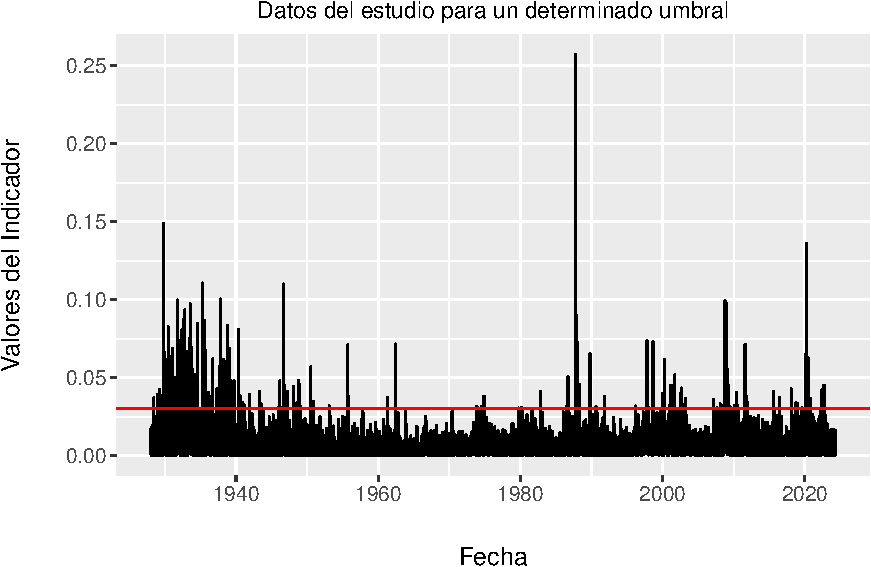
\includegraphics{Entrega_files/figure-latex/unnamed-chunk-32-1.pdf}

\begin{Shaded}
\begin{Highlighting}[]
\CommentTok{\# Paso 3}
\NormalTok{y}\OtherTok{\textless{}{-}}\NormalTok{ Obs[exceso] }\SpecialCharTok{{-}}\NormalTok{ umbral }\CommentTok{\# Esto es lo que llamamos "evento"}
\FunctionTok{length}\NormalTok{(y)}
\end{Highlighting}
\end{Shaded}

\begin{verbatim}
[1] 396
\end{verbatim}

\begin{Shaded}
\begin{Highlighting}[]
\FunctionTok{hist}\NormalTok{(y)}
\end{Highlighting}
\end{Shaded}

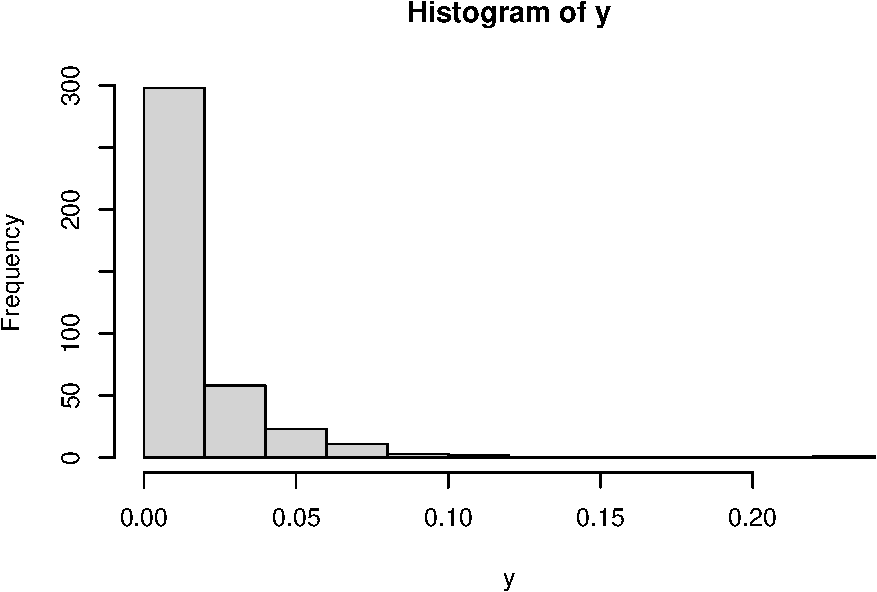
\includegraphics{Entrega_files/figure-latex/unnamed-chunk-34-1.pdf}

Ahora, realizo la prueba de ADF sobre los eventos (datos que están por
encima del umbral) para evaluar la posible presencial de raíz unitaria
para este conjunto de datos.

\begin{verbatim}
Augmented Dickey-Fuller Test 
alternative: stationary 
 
Type 1: no drift no trend 
     lag    ADF p.value
[1,]   0 -11.84    0.01
[2,]   1  -7.33    0.01
[3,]   2  -5.82    0.01
[4,]   3  -5.25    0.01
[5,]   4  -4.35    0.01
[6,]   5  -4.31    0.01
Type 2: with drift no trend 
     lag    ADF p.value
[1,]   0 -16.47    0.01
[2,]   1 -10.92    0.01
[3,]   2  -9.20    0.01
[4,]   3  -8.77    0.01
[5,]   4  -7.61    0.01
[6,]   5  -7.95    0.01
Type 3: with drift and trend 
     lag    ADF p.value
[1,]   0 -16.49    0.01
[2,]   1 -10.95    0.01
[3,]   2  -9.23    0.01
[4,]   3  -8.81    0.01
[5,]   4  -7.65    0.01
[6,]   5  -8.00    0.01
---- 
Note: in fact, p.value = 0.01 means p.value <= 0.01 
\end{verbatim}

\begin{Shaded}
\begin{Highlighting}[]
\FunctionTok{summary}\NormalTok{(}\FunctionTok{ur.kpss}\NormalTok{(y, }\AttributeTok{type =} \StringTok{"mu"}\NormalTok{, }\AttributeTok{lags =} \StringTok{"short"}\NormalTok{,}
        \AttributeTok{use.lag =} \ConstantTok{NULL}\NormalTok{))}
\end{Highlighting}
\end{Shaded}

\begin{verbatim}

####################### 
# KPSS Unit Root Test # 
####################### 

Test is of type: mu with 5 lags. 

Value of test-statistic is: 0.0849 

Critical value for a significance level of: 
                10pct  5pct 2.5pct  1pct
critical values 0.347 0.463  0.574 0.739
\end{verbatim}

\begin{Shaded}
\begin{Highlighting}[]
\FunctionTok{require}\NormalTok{(POT)}
\end{Highlighting}
\end{Shaded}

\begin{Shaded}
\begin{Highlighting}[]
\FunctionTok{length}\NormalTok{(y)}
\end{Highlighting}
\end{Shaded}

\begin{verbatim}
[1] 396
\end{verbatim}

\begin{Shaded}
\begin{Highlighting}[]
\CommentTok{\#i Separamos la muestra para el test de ajuste}
\NormalTok{d}\OtherTok{=} \FunctionTok{round}\NormalTok{(}\FunctionTok{length}\NormalTok{(y)}\SpecialCharTok{*}\FloatTok{0.01}\NormalTok{,}\DecValTok{0}\NormalTok{) }\CommentTok{\# Numero de datos para muestra A (entrenamiento)}

\NormalTok{selA}\OtherTok{\textless{}{-}} \DecValTok{1}\SpecialCharTok{:}\NormalTok{d}

\NormalTok{yA}\OtherTok{\textless{}{-}}\NormalTok{y[selA] }\CommentTok{\# Muestra entrenamiento}
\NormalTok{yB}\OtherTok{\textless{}{-}}\NormalTok{y[}\SpecialCharTok{{-}}\NormalTok{selA] }\CommentTok{\# muestra prueba}

\CommentTok{\# ii{-} ajusto a la muestra A por método de los momentos}
\NormalTok{pwuA }\OtherTok{\textless{}{-}} \FunctionTok{fitgpd}\NormalTok{(yA, }\DecValTok{0}\NormalTok{, }\StringTok{"pwmu"}\NormalTok{)}
\NormalTok{sigmaMomA}\OtherTok{\textless{}{-}}\NormalTok{pwuA}\SpecialCharTok{$}\NormalTok{fitted.values[}\DecValTok{1}\NormalTok{] }\CommentTok{\# scale}
\NormalTok{kMomA}\OtherTok{\textless{}{-}}\NormalTok{pwuA}\SpecialCharTok{$}\NormalTok{fitted.values[}\DecValTok{2}\NormalTok{]  }\CommentTok{\# Shape}

\FunctionTok{cat}\NormalTok{(}\StringTok{"scale:"}\NormalTok{, }\FunctionTok{round}\NormalTok{(sigmaMomA,}\DecValTok{3}\NormalTok{), }\StringTok{"shape:"}\NormalTok{, }\FunctionTok{round}\NormalTok{(kMomA,}\DecValTok{3}\NormalTok{))}
\end{Highlighting}
\end{Shaded}

\begin{verbatim}
scale: 0.012 shape: -0.595
\end{verbatim}

\begin{Shaded}
\begin{Highlighting}[]
\FunctionTok{length}\NormalTok{(yB)}
\end{Highlighting}
\end{Shaded}

\begin{verbatim}
[1] 392
\end{verbatim}

\begin{Shaded}
\begin{Highlighting}[]
\CommentTok{\# iii}
\CommentTok{\#r=2}
\NormalTok{k}\OtherTok{=}\DecValTok{10}
\CommentTok{\# Separamos en 15 grupos }
\NormalTok{yBsplit}\OtherTok{\textless{}{-}}\FunctionTok{split}\NormalTok{(yB, }\DecValTok{0}\SpecialCharTok{:}\FunctionTok{length}\NormalTok{(yB) }\SpecialCharTok{\%/\%}\NormalTok{ k)}
\end{Highlighting}
\end{Shaded}

\begin{verbatim}
Warning in split.default(yB, 0:length(yB)%/%k): data length is not a multiple
of split variable
\end{verbatim}

\begin{Shaded}
\begin{Highlighting}[]
\NormalTok{yBsplit[[}\DecValTok{1}\NormalTok{]]}
\end{Highlighting}
\end{Shaded}

\begin{verbatim}
 [1] 0.007964480 0.008016531 0.008407336 0.013177892 0.006251692 0.010028872
 [7] 0.032781957 0.003009724 0.118636812 0.083068988
\end{verbatim}

\begin{Shaded}
\begin{Highlighting}[]
\FunctionTok{ks.test}\NormalTok{(yBsplit[[}\DecValTok{1}\NormalTok{]] ,}\StringTok{"pgpd"}\NormalTok{,}\AttributeTok{scale=}\NormalTok{sigmaMomA,}\AttributeTok{shape=}\NormalTok{kMomA)}\SpecialCharTok{$}\NormalTok{statistic}
\end{Highlighting}
\end{Shaded}

\begin{verbatim}
        D 
0.3682378 
\end{verbatim}

\begin{Shaded}
\begin{Highlighting}[]
\NormalTok{Tes}\OtherTok{\textless{}{-}}\FunctionTok{unlist}\NormalTok{(}\FunctionTok{lapply}\NormalTok{(yBsplit, }\ControlFlowTok{function}\NormalTok{(X) }\FunctionTok{ks.test}\NormalTok{(X,}\StringTok{"pgpd"}\NormalTok{,}\AttributeTok{scale=}\NormalTok{sigmaMomA,}\AttributeTok{shape=}\NormalTok{kMomA)}\SpecialCharTok{$}\NormalTok{statistic) )}

\NormalTok{T}\OtherTok{\textless{}{-}}\NormalTok{Tes[}\DecValTok{1}\NormalTok{]}
\NormalTok{T\_otros}\OtherTok{\textless{}{-}}\NormalTok{ Tes[}\SpecialCharTok{{-}}\DecValTok{1}\NormalTok{]}

\FunctionTok{hist}\NormalTok{(T\_otros)}
\FunctionTok{abline}\NormalTok{(}\AttributeTok{v=}\NormalTok{T)}
\end{Highlighting}
\end{Shaded}

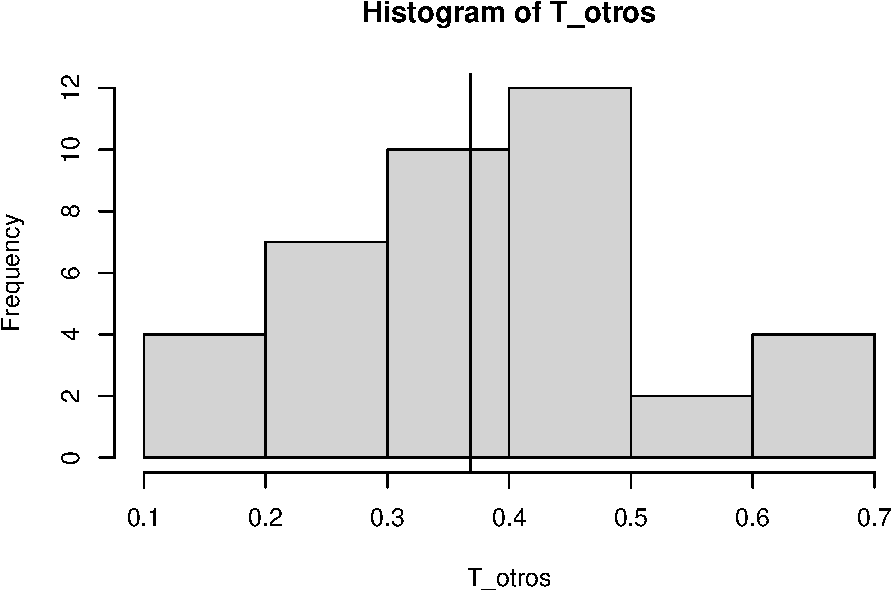
\includegraphics{Entrega_files/figure-latex/unnamed-chunk-44-1.pdf}

\begin{Shaded}
\begin{Highlighting}[]
\FunctionTok{sum}\NormalTok{(T}\SpecialCharTok{\textgreater{}}\NormalTok{T\_otros)}\SpecialCharTok{/}\FunctionTok{length}\NormalTok{(T\_otros)}
\end{Highlighting}
\end{Shaded}

\begin{verbatim}
[1] 0.4102564
\end{verbatim}

\begin{Shaded}
\begin{Highlighting}[]
\NormalTok{pwuTot }\OtherTok{\textless{}{-}} \FunctionTok{fitgpd}\NormalTok{(y, }\DecValTok{0}\NormalTok{, }\StringTok{"pwmu"}\NormalTok{)}
\NormalTok{sigmaMomTot}\OtherTok{\textless{}{-}}\NormalTok{pwuTot}\SpecialCharTok{$}\NormalTok{fitted.values[}\DecValTok{1}\NormalTok{] }\CommentTok{\# scale}
\NormalTok{kMomTot}\OtherTok{\textless{}{-}}\NormalTok{pwuTot}\SpecialCharTok{$}\NormalTok{fitted.values[}\DecValTok{2}\NormalTok{]  }\CommentTok{\# Shape}

\NormalTok{sigmaMomTot}
\end{Highlighting}
\end{Shaded}

\begin{verbatim}
     scale 
0.01112617 
\end{verbatim}

\begin{Shaded}
\begin{Highlighting}[]
\NormalTok{kMomTot}
\end{Highlighting}
\end{Shaded}

\begin{verbatim}
    shape 
0.2897177 
\end{verbatim}

\begin{Shaded}
\begin{Highlighting}[]
\FunctionTok{hist}\NormalTok{(y, }\AttributeTok{prob=}\NormalTok{T)}
\FunctionTok{lines}\NormalTok{(}\FunctionTok{seq}\NormalTok{(}\DecValTok{0}\NormalTok{,}\DecValTok{1}\NormalTok{, }\AttributeTok{length=}\DecValTok{100}\NormalTok{),}\FunctionTok{dgpd}\NormalTok{(}\FunctionTok{seq}\NormalTok{(}\DecValTok{0}\NormalTok{,}\DecValTok{1}\NormalTok{, }\AttributeTok{length=}\DecValTok{100}\NormalTok{), }\DecValTok{0}\NormalTok{, sigmaMomTot,kMomTot))}
\end{Highlighting}
\end{Shaded}

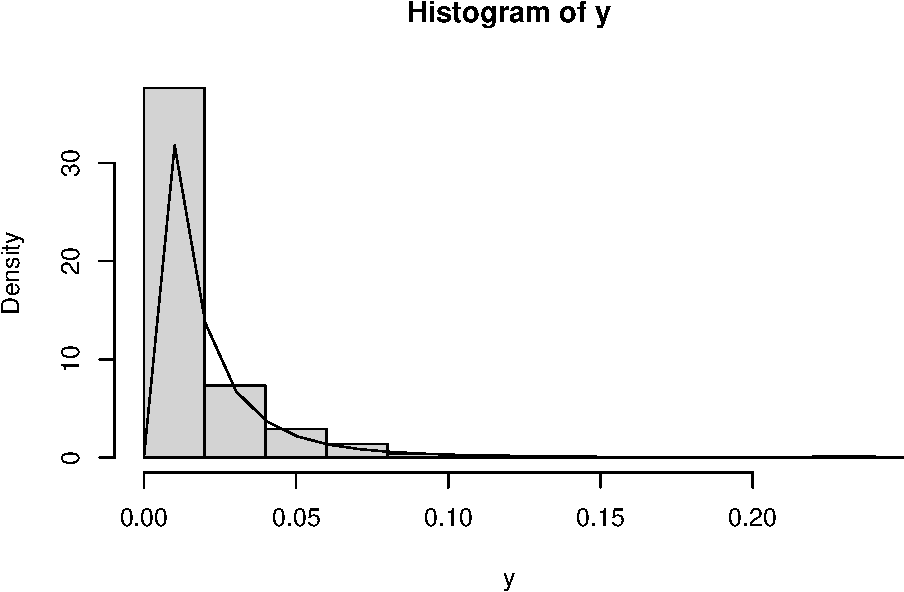
\includegraphics{Entrega_files/figure-latex/unnamed-chunk-48-1.pdf}

\begin{Shaded}
\begin{Highlighting}[]
\CommentTok{\# Ajusto a toda la serie}
\NormalTok{DPGDatos }\OtherTok{\textless{}{-}} \FunctionTok{fitgpd}\NormalTok{(y, }\DecValTok{0}\NormalTok{, }\StringTok{"pwmu"}\NormalTok{)}
\NormalTok{sigmatot}\OtherTok{=}\NormalTok{DPGDatos}\SpecialCharTok{$}\NormalTok{fitted.values[}\StringTok{"scale"}\NormalTok{]}
\NormalTok{ktot}\OtherTok{=}\NormalTok{DPGDatos}\SpecialCharTok{$}\NormalTok{fitted.values[}\StringTok{"shape"}\NormalTok{] }\CommentTok{\# shape}
\end{Highlighting}
\end{Shaded}

\begin{Shaded}
\begin{Highlighting}[]
\NormalTok{umbral}
\end{Highlighting}
\end{Shaded}

\begin{verbatim}
[1] 0.03
\end{verbatim}

\begin{Shaded}
\begin{Highlighting}[]
\CommentTok{\#Con el modelo ajustado podemos pasar a analizar la distribución de los excesos.}
\NormalTok{t}\OtherTok{=}\FloatTok{0.05}
\CommentTok{\# Probabilidad de no exceder un valor mayor a t (t\textgreater{}u)}
\NormalTok{p }\SpecialCharTok{+}\NormalTok{ (}\DecValTok{1}\SpecialCharTok{{-}}\NormalTok{p)}\SpecialCharTok{*} \FunctionTok{pgpd}\NormalTok{(t}\SpecialCharTok{{-}}\NormalTok{umbral, }\DecValTok{0}\NormalTok{, }\FunctionTok{unname}\NormalTok{(sigmatot),}\FunctionTok{unname}\NormalTok{(ktot))}
\end{Highlighting}
\end{Shaded}

\begin{verbatim}
[1] 0.991921
\end{verbatim}

\begin{Shaded}
\begin{Highlighting}[]
\CommentTok{\# Probabilidad de exceder t (el complemento)}
\DecValTok{1} \SpecialCharTok{{-}}\NormalTok{ p }\SpecialCharTok{+}\NormalTok{ (}\DecValTok{1}\SpecialCharTok{{-}}\NormalTok{p)}\SpecialCharTok{*} \FunctionTok{pgpd}\NormalTok{(t}\SpecialCharTok{{-}}\NormalTok{umbral, }\DecValTok{0}\NormalTok{, }\FunctionTok{unname}\NormalTok{(sigmatot),}\FunctionTok{unname}\NormalTok{(ktot))}
\end{Highlighting}
\end{Shaded}

\begin{verbatim}
[1] 0.06059946
\end{verbatim}

\begin{Shaded}
\begin{Highlighting}[]
\DecValTok{1}\SpecialCharTok{{-}} \FunctionTok{sum}\NormalTok{(Obs}\SpecialCharTok{\textless{}}\NormalTok{t)}\SpecialCharTok{/}\FunctionTok{length}\NormalTok{(Obs)}
\end{Highlighting}
\end{Shaded}

\begin{verbatim}
[1] 0.008498092
\end{verbatim}

\paragraph{Procesos estacionarios debilmente
dependientes}\label{procesos-estacionarios-debilmente-dependientes}

\begin{Shaded}
\begin{Highlighting}[]
\FunctionTok{library}\NormalTok{(TSA)}
\end{Highlighting}
\end{Shaded}

\begin{verbatim}

Attaching package: 'TSA'
\end{verbatim}

\begin{verbatim}
The following objects are masked from 'package:stats':

    acf, arima
\end{verbatim}

\begin{verbatim}
The following object is masked from 'package:utils':

    tar
\end{verbatim}

\begin{Shaded}
\begin{Highlighting}[]
\FunctionTok{library}\NormalTok{(tseries)}
\end{Highlighting}
\end{Shaded}

Evaluemos la independencia de la serie con un test de rachas. Recuerden
que existen varios test para evaluar aleatoriedad, ver el Lab 2 para más
ejemplos. Este procedimiento deben realizarlo para todos los casos
(incluidos los anteriores).

\begin{Shaded}
\begin{Highlighting}[]
\NormalTok{ts\_relacion}\SpecialCharTok{$}\NormalTok{Date}\OtherTok{=}\FunctionTok{row.names}\NormalTok{(ts\_relacion)}
\NormalTok{ts\_relacion}\SpecialCharTok{$}\NormalTok{Date}\OtherTok{=}\FunctionTok{as.Date}\NormalTok{(ts\_relacion}\SpecialCharTok{$}\NormalTok{Date)}
\end{Highlighting}
\end{Shaded}

\begin{Shaded}
\begin{Highlighting}[]
\FunctionTok{acf}\NormalTok{(ts\_relacion}\SpecialCharTok{$}\NormalTok{indicador)}
\end{Highlighting}
\end{Shaded}

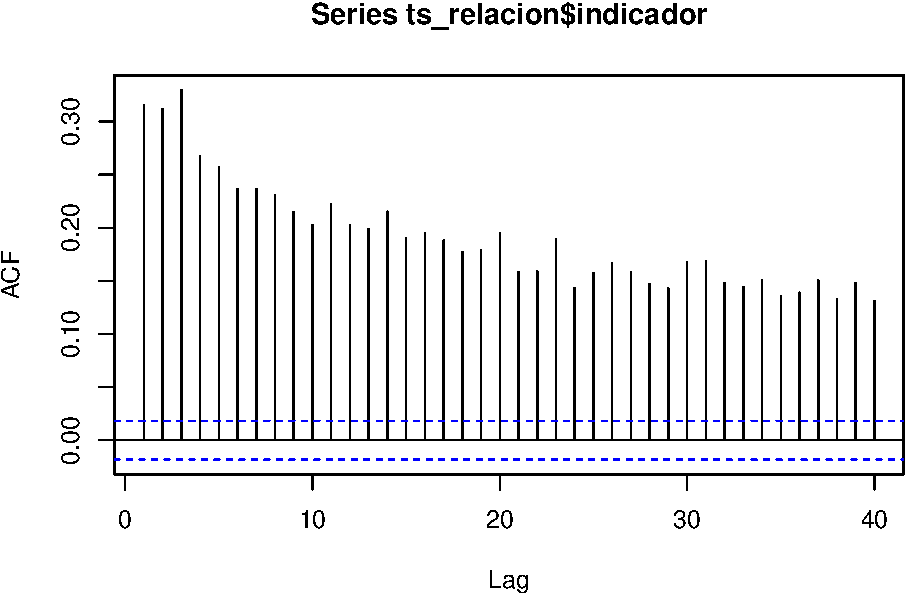
\includegraphics{Entrega_files/figure-latex/unnamed-chunk-56-1.pdf}

\begin{Shaded}
\begin{Highlighting}[]
\FunctionTok{runs.test}\NormalTok{(}\FunctionTok{as.factor}\NormalTok{(ts\_relacion}\SpecialCharTok{$}\NormalTok{indicador}\SpecialCharTok{\textgreater{}}\FunctionTok{median}\NormalTok{(ts\_relacion}\SpecialCharTok{$}\NormalTok{indicador)))}
\end{Highlighting}
\end{Shaded}

\begin{verbatim}

    Runs Test

data:  as.factor(ts_relacion$indicador > median(ts_relacion$indicador))
Standard Normal = -14.937, p-value < 2.2e-16
alternative hypothesis: two.sided
\end{verbatim}

El resultado (p-valor muy pequeño) indica que no estamos en condiciones
de asumir aleatoriedad en los datos. Veamos que pasa si consideramos
datos sobre cierto umbral.

\begin{Shaded}
\begin{Highlighting}[]
\NormalTok{tsq90}\OtherTok{=}\FunctionTok{quantile}\NormalTok{(ts\_relacion}\SpecialCharTok{$}\NormalTok{indicador,}\FloatTok{0.90}\NormalTok{)}
\NormalTok{tsq90}
\end{Highlighting}
\end{Shaded}

\begin{verbatim}
       90% 
0.01756989 
\end{verbatim}

\begin{Shaded}
\begin{Highlighting}[]
\NormalTok{ts}\OtherTok{=}\NormalTok{ts\_relacion}\SpecialCharTok{$}\NormalTok{indicador}
\NormalTok{exceso\_ts}\OtherTok{\textless{}{-}}\FunctionTok{which}\NormalTok{(ts }\SpecialCharTok{\textgreater{}}\NormalTok{ tsq90)}
\FunctionTok{length}\NormalTok{(exceso\_ts)}
\end{Highlighting}
\end{Shaded}

\begin{verbatim}
[1] 1154
\end{verbatim}

Evaluemos la aleatoriedad sobre los excesos.

\begin{Shaded}
\begin{Highlighting}[]
\NormalTok{ts\_e}\OtherTok{=}\NormalTok{ts[exceso\_ts]}
\FunctionTok{runs.test}\NormalTok{(}\FunctionTok{as.factor}\NormalTok{(ts\_e}\SpecialCharTok{\textgreater{}}\FunctionTok{median}\NormalTok{(ts\_e)))}
\end{Highlighting}
\end{Shaded}

\begin{verbatim}

    Runs Test

data:  as.factor(ts_e > median(ts_e))
Standard Normal = -4.5353, p-value = 5.752e-06
alternative hypothesis: two.sided
\end{verbatim}

\newpage

\section{Referencias bibliográficas}

\phantomsection\label{refs}
\begin{CSLReferences}{1}{0}
\bibitem[\citeproctext]{ref-notas_curso}
Crisci, C., Perera, G., \& Segura, A. (2021). \emph{Curso de estadística
de datos extremales, cap. 1 a cap. 5}.

\bibitem[\citeproctext]{ref-enders}
Enders, W. (2014). \emph{Applied Econometric Time Series}. Wiley.

\bibitem[\citeproctext]{ref-kpss}
Shin, Y., Kwiatkowski, D., Schmidt, P., \& Phillips, P. C. B. (1992).
Testing the Null Hypothesis of Stationarity Against the Alternative of a
Unit Root: How Sure Are We That Economic Time Series Are Nonstationary?
\emph{Journal of Econometrics}, \emph{54}(1-3), 159-178.

\bibitem[\citeproctext]{ref-evd}
Stephenson, A. G. (2002). evd: Extreme Value Distributions. \emph{R
News}, \emph{2}(2), 0. \url{https://CRAN.R-project.org/doc/Rnews/}

\end{CSLReferences}

\newpage

\section{Appendix}\label{appendix}

\end{document}
